\chapter{Introduction}
\minitoc
This document describes \ggn, a software layer that
establishes usage standards and software tools for building 
\href{http://www.earthsystemmodeling.org}{ESMF}
compliant components. This package
\begin{enumerate}
\item facilitates the porting of existing codes to ESMF
\item provides tools and a straightforward recipe for building new ESMF
components, and
\item provides much greater interoperability between compliant
components than between current ESMF compliant components (!?!?!).
\end{enumerate}

As the Earth System Modeling Framework (ESMF)
has become available, several groups have been involved in prototyping
its use in climate and weather prediction models and in data
assimilation systems.  Existing programs have been converted to use
the superstructure of the framework at MIT, NCAR, GFDL, Goddard,
NCEP and the DoD (see 
\href{http://www.earthsystemmodeling.org/impacts/index.shtml}{impacts}).
One of the
most complete attempts to use ESMF has been the development of the
\href{http://geos5.org}{GEOS-5} AGCM, a model targeted by the
\href{http://map.nasa.gov}{MAP announcement}. GEOS-5 has been
built `from the ground up' using the latest available versions of ESMF
superstructure and infrastructure. Figure \ref{fig:geos5_esmf} represents a
hierarchical (tree) implementation of the component-based GEOS-5 software
where each box is an ESMF component performing some specific function and
the root of the tree serves as the top level control point.
%
\begin{figure}[h]
  \label{fig:geos5_esmf}
  \centering
  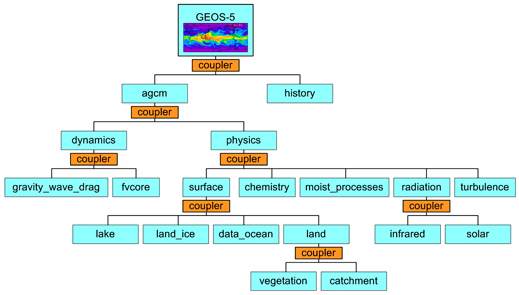
\includegraphics[scale=0.75]{figs/geos5_esmf.jpg}
  \caption{Structure of the GEOS-5 atmospheric general circulation model}
\end{figure}
%

All of these efforts have produced much constructive feedback to the
ESMF core development team, and have helped refine the design and
improve the implementation of the framework. They have also served to
identify the most important directions for future extensions.
Comparing the various implementations led to two seemingly
contradictory conclusions: all implementations are different and
much of what they do is the same.  Both conclusions were
anticipated, since ESMF is a general framework designed to meet a wide
variety of needs.  This generality is an important strength of the
ESMF design, but it also implies that there are many different ways of
using ESMF - even when performing very similar tasks. Other
observations from this early experience were that each group, within
its own implementations, \emph{repeatedly} needed functions that provided
higher level functionality than that provided by the basic ESMF tools,
and that \emph{the core methods of ESMF components ({\tt Run}, 
{\tt Initialize}, and {\tt Finalize}) looked very similar in all
their implementations}.

The \ggn\ package arose as a response to this early
experience, particularly during the construction of GEOS-5.
It is based on the observation that much of the work done in these initial
implementations can be standardized; thus, reducing the labor of
constructing ESMF applications in the future, as well as increasing
their interoperability. In its initial implementation, \ggn\  
provides:
%
\begin{itemize}
\item Specific conventions and best practices for the utilization 
of ESMF in climate models
\item  A middle-ware layer (between the model and ESMF) that
facilitates the adoption of ESMF by climate models.
\end{itemize}

This enhancement in usability of ESMF must come at the cost of reduced
generality. To make the framework more usable for our applications, we
make assumptions and place requirements on the applications that ESMF,
with its goal of generality, could not. \ggn\ does this 
`on top of' ESMF and as a separate layer through which the
application uses ESMF for some of its functions (although for most
things, applications will continue to use ESMF directly). We feel that
this middle-ware-layer approach is the right way to get the usability
and interoperability that climate model components require of the
framework, without sacrificing ESMF's generality and extensibility.

The documentation is arranged as follows: In Chapter 2, we review
relevant aspects of ESMF, followed by a chapter that aims to introduce
readers, already familiar with ESMF, quickly into \ggn\ through examples
that increase in complexity, demonstrating the salient features of \ggn.
The following chapter provides are more detailed description of \ggn\
followed by the \ggn\ API (Application Programming Interface) and the
source codes for tutorials in the appendix.


\chapter{ESMF - A review of aspects relevant to MAPL}
\minitoc

\textbf{Leaf and Composite components are defined here}.


The Earth System Modeling Framework (ESMF) \cite{deluca} is a
software package designed to provide some of the essential functions
needed by parallel, scalable earth system models in a
machine-independent way. ESMF is implemented as a collection of very
general programming classes that can be used both to construct ESMF
components and to connect them to one another.
These classes thus support modelers in
building interoperable and portable codes. This design is illustrated
by the ESMF `sandwich' diagram (Figure \ref{fig:esmf_sandwich}), where the
user's computational code sits between the two ESMF layers.
%
\begin{figure}[h]
  \label{fig:esmf_sandwich}
  \caption{Schematic of the ESMF `sandwich' architecture. The
    framework consists of two parts, an upper level superstructure
    layer and a lower level infrastructure layer. User code is
    sandwiched between these two layers. Taken from \cite{esmfManual}}.
  \centering
  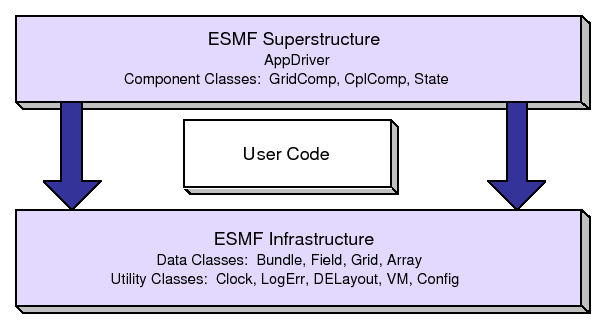
\includegraphics[scale=0.7]{figs/esmf_sandwich.png}
\end{figure}
%

The simplest ESMF implementation consists of building a Gridded
Component (an ESMF superstructure class) that encapsulates the user
code, interfacing it to the framework by defining the ESMF callable
methods (\texttt{Initialize}, \texttt{Run} and \texttt{Finalize},
hereafter, \IRF\ methods). This
can actually be done without using any of the ESMF Infrastructure - a
strategy that fails to capitalize on some of ESMF's greatest
strengths. Such `encapsulation' implementations have dominated the early
adoptions of ESMF.

More sophisticated implementations put user data in ESMF
infrastructure objects (primarily \fld s) which can then be
manipulated by a wide array of ESMF methods to facilitate the coupling
of components with different data structures (i.e., that are on
different grids) and to insulate the user
from the architecture-specific implementation layers that are used for
inter-process or inter-processor communication, I/O, etc.

An ESMF component (represented by a box in Figure \ref{fig:geos5_esmf},
e.g. \texttt{solar}) consists of four (\textbf{or just one --- SetServices!?!?!}) public component interface functions
performing specific roles:
\begin{description}
\item[\ssv:] A component's \ssv\ function is called when an
instance (object) of the component is created and is the \emph{only required
public interface} of the component. It takes the instantiated component as
the first argument, and an integer return code as the second. The goal of
\ssv\ is to register with the framework the component's user-defined routines
that satisfy the \texttt{Initialize}, \texttt{Run} and \texttt{Finalize}
requirements.
\item[\texttt{Initialize}:] A component's \texttt{Initialize} function
is called to configure an instance (object) of the component (allocate
space, initialize data etc.). In addition to
the component's instance, the arguments to this function include two
\stt s (one \im\ and one \ex) and an \texttt{ESMF\_Clock}. The \stt\
variables are used to pass data between components. The
\texttt{Clock} is used to pass the simulation time counter to the component
instance.
\item[\texttt{Run}:] A component's \texttt{Run} function is called to
carry out a cycle of the iteration that makes up the kernel of a component's
computational algorithm. This function contains the kernel of user code
and is called repeatedly as part of the
component instance's life cycle. It takes the same argument list as
\texttt{Initialize}.
\item[\texttt{Finalize}:] A component's \texttt{Finalize} function is
called to terminate the the component instance cleanly (release space,
write results etc.). It takes the same argument list as \texttt{Initialize}.
\end{description}

Some important aspects of the ESMF API that are relevant to
\ggn\ are:
%
\begin{itemize}
\item Data structures added to an \stt\ can have \emph{arbitrary meta tags}
  associated with them
\item An \stt\ can contain an \stt\ variable allowing \emph{recursive nesting}
  of \stt\ variables.
\item \emph{Hierarchical organization of gridded components}: \egc s can be
simple containers for user code (leaf components) or they can contain other
gridded \egc s (composite components). The notion of composite components
allows a straightforward way of organizing applications as a hierarchy of
components. ESMF does not require a hierarchical organization, but it is
the most natural way of connecting ESMF components.
\item ESMF also defines the notion of \emph{Coupler Components}.
These are similar to gridded components, but are not intended for user code;
rather, they house the transformations necessary to convert between \ex s
of one component and \im s of another.
\end{itemize}

In designing ESMF, a deliberate decision was made to have the
framework provide these services in a very general way, and not to
prejudge how future models would use it or what programming models
would best suit future computer architectures. This generality is an
important strength of ESMF, but it is also an impediment to many users
that would prefer a more specific formulation for porting existing
codes or a better defined recipe for building new codes with ESMF. The
generality also impacts the interoperability of applications, since
the ESMF interfaces to the \IRF\ methods are general purpose, and they
carry little information (other than the grid definition) about the
physical content of the data moving in and out of the gridded
component.

The middle-ware layer implemented in \ggn\  includes the following
design elements:
%
\begin{enumerate}
%
\item Aides in constructing a component's \IRF\ methods

\item Provides easy-to-use tools for describing the contents of a
  component's \im\ and \ex\ states, as well as adopting conventions for what
  must be described. But in no way specifying what the contents must be.
  \ggn\ extends the \stt\  concept to a component's \gin\ state, and
  help it manage its persistent data.
  
\item Facilitates the use of \fld s and thus of the ESMF 
  Infrastructure layer

\item Facilitates the coupling of components into complex applications. This
  requires a means of describing the connectivity between components and
  of using the description of the \im\ and \ex\ states to couple
  components - \ggn\ adopts the hierarchical organization as its
  architecture for making complex applications and uses both composite
  gridded components and ESMF coupler components to establish connections
  between members of the hierarchy.
\end{enumerate}



% \chapter{MAPL - Quickstart}
% \minitoc
% The goal of this chapter is to introduce the reader already familiar
% with ESMF, quickly to MAPL through examples increasing in complexity
% and demonstrating various features of \ggn. Also much of the code
% presented here can be easily adapted to write application-specific
% gridded components.

% It is assumed that the user already has an account on
% \href{https://www.nccs.nasa.gov/discover_front.html}{NCCS discover} with
% access to the source code repository (see progress repository
% \href{https://progress.nccs.nasa.gov/trac/admin/wiki/QuickStart}{quickstart}
% - the link requires NCCS username and password). Also the shell is assumed
% to be \texttt{csh}.

% In the following, for the sake of brevity, we have skipped verification
% of the return code from functions/subroutines. For production codes,
% it is highly advisable that every call to an ESMF or \ggn\ routine
% (for that matter any fortran routine supplying a return code e.g.
% \texttt{allocate}/\texttt{deallocate} etc.) should be followed
% by a statement like
% \begin{verbatim}
%     _VERIFY(stat)
% \end{verbatim}
% where \texttt{VERIFY\_} is a \ggn\ utility and \texttt{stat} is an
% \texttt{integer} return code.

% \section{Build and Run}

% The first step is to check out the tutorial module from the CVS repository.
% Once the CVS environment has been set up, the module can be pulled from
% the repository.
% \begin{verbatim}
%   $ setenv CVS_RSH ssh
%   $ setenv CVSROOT :ext:USERID@cvsacl:/cvsroot/esma
%   $ cd /discover/nobackup/USERID
%   $ cvs co -r mapl_doc G5tutorial
% \end{verbatim}
% Here \texttt{USERID} is the NCCS username. 

% Next step is to compile the module. For NCCS discover, a
% script (\texttt{g5\_modules}) is provided to create the necessary
% environment for running and compiling. Once the required modules have been
% loaded and the environment variable \texttt{BASEDIR} has been set, the
% examples can be built.
% \begin{verbatim}
%   $ cd G5tutorial/src
%   $ source g5_modules
%   $ make install
% \end{verbatim}
% This creates the following executables in the
% \texttt{G5tutorial/src/Applications/Examples} directory:
% \begin{verbatim}
%   ex001-CFIO_Array.x
%   ex002-CFIO_Bundle.x 
%   ex003-FieldBundle.x
%   ex004-Config.x
%   ex005-GridComp.x 
% \end{verbatim}

% All of these examples assume 2 processors, and so are typically run as
% \begin{verbatim}
%   $ xsub -I
%   $ mpirun -np 2 ./executable_name
% \end{verbatim}

% The command `\texttt{xsub -I}' starts an
% \href{http://www.nccs.nasa.gov/primer/computing.html#interactive}
% {interactive batch} on NCCS discover (with x forwarding).

% \section{Example - Creating grids and reading arrays from files}
% \label{sec:exgrid}
% This section demonstrates, using a simple ESMF/\ggn\ example, how to
% \begin{enumerate}
% \item Initialize ESMF
% \item Create a grid and retrieve latitudes/longitudes
% \item Use time manager to create a time object
% \item Read 2D and 3D arrays from a file
% \item Read data with automatic time interpolation
% \end{enumerate}

% The source code is available at:\\
% \texttt{G5tutorial/src/Applications/Examples/ex001-CFIO\_Array.F90}.
% Below, we provide a description of the code. For line numbers,
% please refer to the listing of the code in \ref{sec:tutex1}.
% \begin{description}
% \item[lines 21-22] We always have these, for ESMF/\ggn\ applications.
% \item[lines 28-58] Declare variables, including 3D/2D grids, time objects,
%   file names, arrays to hold data read from file, coordinate variables,
%   Iam (\textbf{explain!?!?!}).
% \item[line 60] \texttt{Main()} does the actual work, so call it.
% \item[lines 69-80] Initialize ESMF (turn off ESMF's automatic logging
%   feature for greater performance). Get the total number of processes
%   as well as the local process number. Make sure, we are using 2 processes.
%   Here \texttt{\_\_RC\_\_} is a macro, defined in \texttt{MAPL\_Exceptions.h},
%   that is an automatic exception handler for \texttt{rc=STATUS}.
% \item[lines 91-93] Create a 3D lat-long grid, \texttt{grid}, on a 2x1 layout
%   (\textbf{what is that!?!?!}).
% \item[lines 98-100] Similarly, create a 2D grid, \texttt{grid2d}.
% \item[lines 104-105] Retrieve \texttt{lons} and \texttt{lats} from the 3D grid.
% \item[lines 109-110] Get local dimensions, \texttt{im}, \texttt{jm},
%   \texttt{km}, from the 3D grid.
% \item[lines 114-118] Set time as the one of the hardwired file names
%   (\textbf{!?!?! this I don't get}).
% \item[lines 126-131] Read 2D arrays from file and store them.
% \item[lines 135-138] Read 3D arrays from file and store them.
% \end{description}
% \emph{Next, we test automatic time interpolation}:
% \begin{description}
% \item[lines 143-145] Set 3 \texttt{ESMF\_Time} objects to
%   (1) 03/16/2001-12:00:00, (2) 03/31/2001-18:00:00 and (3) 04/16/2001-00:00:00
%   (format: mm/dd/yyyy-HH:MM:SS).
% \item[lines 150-156] Read 3D \texttt{CH4} data from file at three different
%   times (set in the previous step) (\textbf{is this correct!?!?!}).
% \item[lines 171-172] If root, compute mean of the \texttt{CH4} data at
%   times 1 and 3 and compute the absolute error from \texttt{CH4} data at time 2.
% \item[line 188] Compute and print the Root Mean Square error.
% \item[line 197] Finalize ESMF.
% \end{description}

% \section{Example - Bundle operations including read/write}
% \label{sec:exbundleops}
% This section demonstrates, using a simple ESMF/\ggn\ example, how to
% \begin{enumerate}
% \item Initialize ESMF
% \item Create a grid
% \item Use time manager to create a time object
% \item Read bundles from a file
% \item Iterate through items in a bundle
% \item Get Fortran arrays out of a Bundle
% \item Create a new Bundle and populate it with a new Field.
% \end{enumerate}

% The source code is available at:\\
% \texttt{G5tutorial/src/Applications/Examples/ex003a-FieldBundle.F90}.
% Below, we provide a description of the code. For line numbers,
% please refer to the listing of the code in \ref{sec:tutex2}.
% \begin{description}
% \item[lines 98-103] Create a global 2D Lat-Lon grid, \texttt{myGrid},
%   on a 2x1 layout.
% \item[lines 107-108] Set time to 01/01/2001-00:00:00.
% \item[lines 112-113] Create an empty bundle (\texttt{myBundle}) and read
%   all variables from file into it.
% \end{description}
% \emph{Look into the bundle}:
% \begin{description}
% \item[line 122] Root prints a summary of the \texttt{myBundle} contents.
% \item[line 127] Get the number of fields in \texttt{myBundle}.
% \item[line 135] Get the i$^{\rm th}$ field (\texttt{ithField})
%   from \texttt{myBundle}.
% \item[line 139] Get field name of \texttt{ithField}.
% \item[line 143] Get the fortran array (\texttt{Array}) inside \texttt{ithField}.
% \item[line 160] \ggn\ has a routine for getting an array, by name out
%   of a bundle. \texttt{Note}: ESMFL instead of \ggn.
% \end{description}
% \emph{Make a new bundle}:
% \begin{description}
% \item[lines 175-180] Create a new array, \texttt{newArray} to go into
%   the new bundle.
% \item[line 190] Create a new Field, \texttt{newField} by combining
%   \texttt{newArray} and \texttt{myGrid}.
% \item[line 194] Create and empty bundle, \texttt{newBundle}.
% \item[line 198] Store \texttt{newField} into \texttt{newBundle}
% \item[lines 202-210] Get array back from \texttt{newBundle} and check
%   to make sure that we got it right
% \item[lines 215-219] Clean up. Order of cleaning up is important - 
%   the contents of a bundle (e.g. field) should be desctroyed before
%   the bundle is destroyed (\textbf{is this correct!?!?!}).

% \end{description}

% \section{Example - Basic \texttt{ESMF\_Config} usage}
% \label{sec:exesmfconfig}
% This section demonstrates, using a simple ESMF/\ggn\ example, how to
% \begin{enumerate}
% \item Initialize ESMF
% \item Create an ESMF Config object
% \item Illustrate scalar attributes
% \item Illustrate vector parameters
% \item Illustrate the use of tables
% \end{enumerate}

% The source code is available at:\\
% \texttt{G5tutorial/src/Applications/Examples/ex004-Config.F90}.
% Below, we provide a description of the code. For line numbers,
% please refer to the listing of the code in \ref{sec:tutex3}.
% \begin{description}
% \item[lines 80-81] Load a simple resource (configuration) file.
% \end{description}
% \emph{Scalar resources}:
% \begin{description}
% \item[lines 89-91] Get integers \texttt{Nx}, \texttt{Ny} and \texttt{Nz}.
% \item[lines 99-101] Value of an attribute can easily be modified.
% \end{description}
% \emph{Vector resources}:
% \begin{description}
% \item[lines 112-113] Get vectors \texttt{BegDate} and \texttt{EndDate}.
% \end{description}
% \emph{Table with real numbers}:
% \begin{description}
% \item[line 127] Get the dimensions of the table.
% \item[lines 134-138] Read the table.
% \end{description}
% \emph{Variable column table with strings}:
% \begin{description}
% \item[line 151] Get the dimensions of the table.
% \item[lines 158-164] Read the table. Note the double loop here as
%   opposed to the single loop in the case of the fixed sized table.
% \item[line 175] Clean up.
% \end{description} 

% \section{Example - Stand-alone gridded component}
% \label{sec:exstandalonegc}
% This example illustrates a typical use ESMF/\ggn\ to build applications.
% The steps are
% \begin{enumerate}
% \item Initialize ESMF
% \item Create a 2D grid, validate it
% \item Create clock
% \item Create \IM/\EX\ states and the \texttt{gridded component}
% \item Set the component's \ssv\
% \item Initialize component
% \item Run component
% \item Clean up
% \end{enumerate}

% The source codes for this example are:\\
% \texttt{G5tutorial/src/Applications/Examples/ex005-GridComp.F90} and\\
% \texttt{G5tutorial/src/Applications/Examples/Example\_GridComp/Example\_GridCompMod.F90}.

% \texttt{ex005-GridComp.F90} is the driver routine that creates
% a component, and performs its \IRF\ functions
% thorugh the ESMF framework. \texttt{Example\_GridCompMod.F90} implements
% the component's internals, its \emph{only} public routine
% \ssv\ (registering the user-defined \IRF\ routine with ESMF) and
% the user-defined \IRF\ methods themselves.

% Below, we provide a description of the code. For line numbers,
% please refer to the listing of the code in \ref{sec:tutex4}.
% \begin{description}
% \item[lines 96-105] Create a global 2D Lat-Lon grid on a 2x1 layout
%   and validate it (\textbf{what is that!?!?!}).
% \item[lines 109-112] Create clock starting at 01/01/2001 OZ
%   (\textbf{what is OZ!?!?!}) with a 30 minute timestep.
% \item[lines 117-123] Create \IM/\EX\ states and the component \texttt{GC}.
%   Corresponding to \texttt{GC}, the module \texttt{Example\_GridCompMod}
%   (in file \texttt{Example\_GridComp/Example\_GridCompMod.F90}) defines
%   the component's \emph{only public routine} \ssv.
% \item[line 129] Set component's \ssv\ that registers the component's
%   \texttt{Initialize}, \texttt{Run} and \texttt{Finalize} methods with
%   the ESMF framework. The user-defined functions are
%   \texttt{Initialize\_}, \texttt{Run\_} and \texttt{Finalize\_}.
% \item[line 133] Initialize component - this results in a call to the
%   \texttt{Initialize\_} routine by the ESMF framework.
% \item[line 144] Run component - ESMF framework calls \texttt{Run\_}.
% \item[line 148] Finalize component - ESMF framework calls \texttt{Finalize\_}.
% \end{description}

\chapter{MAPL}
\label{ch:mapl}
\minitoc

\section{Overview}
The \ggn \ library can be divided into the following sub-systems:
\begin{description}

\item[\ggn\_Core] is a collection of routines and conventions used to
  build \egc s (or to wrap legacy codes as \egc s). In particular, it
  includes the means of describing a component's \im\ and \ex\ states
  as well as the new \gin\ state.

\item[\ggn\_Connect] is a collection of routines and conventions used for
  organizing \ggn-ESMF Gridded Components into a \ggn\ hierarchy.
  
\item[\ggn\_History] is an ESMF Gridded Component that sits inside MAPL and
  \emph{can} be instantiated to provide data writing services for a MAPL
  hierarchy.

\item[\ggn\_ExtData] is an ESMF Gridded Component that sits inside MAPL and
  \emph{can} be instantiated to provide data services to the IMPORT states
  of MAPL components in a hierarchy.

\item[\ggn\_Utils] is a set of support utillities for commonly performed
  tasks in global climate models. \ggn\ itself uses some of these, but,
  like \ggn\_History, \ggn\ components or applications need not use them.

\item[\ggn\_CFIO] is an I/O layer for ESMF \texttt{Field}s, 
  \texttt{Bundle}s and \texttt{State}s that uses CF (Climate and Forecast)
  compliant methods to read from (or write to) NetCDF, HDF or GrADS files.
  It relies internally on \ggn\ and must be built with it and can be used
  even if one is not using the rest of \ggn.

\end{description}

The distinction between \ggn\_Core and \ggn\_Connect, which in
the \ggn\ code are mostly within the \texttt{MAPL\_Generic} module,
is important. One may use \ggn\_Core alone as a means of facilitating the
introduction of ESMF, with no intention of ever coupling the component to a 
\ggn\  hierarchy. A component so contructed is a perfectly good
ESMF component and, other than having to access the \ggn\  library
to build and execute, is not special in any way. The code in 
an application instantiating it would not need to know it was built 
with \ggn\  machinery.


\section{Building a \ggn\ Gridded Component: \ggn\_Core}

\ggn's original intention, and its core function, is
to provide assistance in writing ESMF Gridded components. It does this
in the following ways:
%
\begin{enumerate} 
%
\item It makes it easier to write a component's \IRF\ methods. In fact
  in some cases they need not be written at all.

\item It adds an \gin\ (\gIN ) \texttt{ESMF\_State}
  to the component, supplementing the \im (\IM ) and \ex (\EX )
  states required by ESMF.

\item It provides a means of describing the contents of the three states
   so that \ggn\  can help manage them.
   
\item It adopts ground rules for the behavior of a component 
  and its treatment of the three states.

\item It defines a standard recipe for writing 
 \ggn -based ESMF Gridded Components.
 
\end{enumerate} 
Each of these items is discussed in more detail in the following subsections.
It will be helpful to refer to the complete \ggn\ example in section
\ref{sec:maplExample}.

\subsection{Writing the \IRF\ method} 
After writing some gridded components, one realizes that, except
the actual insertion of the user code, most \ssv\ and \IRF\
methods are very similar, and that it would be economical to
generalize this `boilerplate' code. \ggn\ provides
three (\textbf{or two!?!?!}) ways of doing this.
%
\begin{enumerate}
\item[a)] The first way is to use the generic versions of 
  \ssv\  and the \IRF\ methods provided by \ggn\ as the 
  component's methods. When \gssv\  is
  invoked, it registers the three Generic \IRF\ methods. If not overridden,
  these become the component's actual methods.
  
\item[b)] A second way of using \ggn\  is to simply call the generic
  versions of the methods from the component-specific versions, allowing
  them to perform the boilerplate functions. 
  
\item[c)] \textbf{Should this really be included!?!?!}
  A third way is to simply use the source code
  of the generic versions as templates for the specific versions.
  Taking this approach is \emph{dangerous and not allowed} for \ggn-compliant
  components. 

\end{enumerate}

So what do the Generic \IRF\ methods do? This will be described in detail
in subsequent sections, but simply stated, they manage the
\IM/\EX\ States and a third \stt\, '\gin'
that we will discuss below. We will refer to these three
states as the \IM/\EX/\gIN\ states. Note that they are all ordinary \stt s.
From the description of the three states (\ref{sec:descStContents})
provided in the data services, \ggn\  is able to create, allocate,
initialize, and destroy all items in these states; it can also
checkpoint and restart the \gin\ and \im\ states. The \IRF\ methods also
implement connectivity of children components, creating the appropriate
couplers, registering their services, and executing their \IRF\ methods.


\subsection{The new \gin\ (\gIN) State}

ESMF requires that the control
is passed back to it at the end of a component's \texttt{Run} method.
In the spirit of having as unintrusive a design as possible,
\emph{ESMF says nothing about a component's internal state} which will
probably be needed during subsequent executions of the component's
\texttt{Run}. \ggn\ provides a mechanism to place parts of its true
internal state in an \stt\, called an \gin\ state, that is similar to the
\IM/\EX\ states.

Since it is desirable that gridded components be as
object-oriented as possible, the framework has to allow them to be fully
instantiatable. This requires that whatever the component defines as
its internal state be \emph{attached} (in the object-oriented paralance)
to the instance of the \egc. ESMF provides such a mechanism - effectively a hook
on which a component can hang the current instance of its internal state.

Accordingly, this new \gIN\ state does not appear explicitly in the argument
list of \IRF\ methods, as is the case with the \IM/\EX\ states; instead
it is \emph{attached} to the \egc\  and, in principle, is accessible only
through \ggn\ and can be queried.

All of the mechanisms for registering and manipulating data that are
already available in \ggn\  for the \IM/\EX\ States, are
extended to the \gIN\ state. The default accessibility rules
for this state are that \emph{its items can be written only by the component
and can be read only by its parent}. All data registered in this state
by the component's \ssv\  are, of course, automatically
allocated, checkpointed, and restarted by the \ggn\ \text{Initialize}
and \texttt{Finalize} methods.


\subsection{Description of State contents} \label{sec:descStContents}
The simplest ESMF gridded component consists of the
\IRF\ methods encapsulating the user's computational code. These
methods are private to the component, but are callable by the
framework; in fact, \emph{they can only be called by the framework}. This
is accomplished by having in each component a public method
(\ssv) that tells the framework what functions it can perform
(initialize the component, run it, etc.). The framework can then
invoke these functional services when they are required.

The interface to these services is prescribed by ESMF and includes
\im\ and \ex\ (\IM/\EX) States, through which all data is exchanged
between the components. These states can contain only ESMF
objects (primarily \fld s and other \stt s),  but ESMF says
nothing about how they are to be used. \ggn\ assumes that
\IM/\EX\ states consist only of \fld s and other \stt s. It also adopts
the convention that, by default, items in its \ex\ state are not
modified by other components and that a component cannot modify items in its
\im\ state (this default behavior can be changed by adding a `FRIENDLY\_TO'
attribute to an \IM\ state).

A major innovation in \ggn\ is a means of describing the
contents of the \IM/\EX\ states. \ggn\ takes the view that
\begin{quote}
\emph{a component, in addition to giving the framework access to its
functional services, should also tell the framework about its data
services, i.e., what it needs from others and what it can provide}.
\end{quote}
\ggn\ extends the use of \ssv\ to accomplish this. The
\ssv\ method of a \ggn-based gridded component will
contain {\em spec calls} like the following:

Adding \im\ state:
\begin{verbatim}
    call MAPL_AddImportSpec  (GC,                                &
                              SHORT_NAME = 'PLE',                &
                              LONG_NAME  = 'air_pressure',       &
                              UNITS      = 'Pa',                 &
                              DIMS       = MAPL_DimsHorzVert,    &
                              VLOCATION  = MAPL_VLocationEdge,   &
                              RC         = STATUS)
\end{verbatim}

Adding \ex\ state:
\begin{verbatim}
    call MAPL_AddExportSpec  (GC,                                &
                              SHORT_NAME = 'U',                  &
                              LONG_NAME  = 'eastward_wind',      &
                              UNITS      = 'm s-1',              &
                              DIMS       = MAPL_DimsHorzVert,    &
                              VLOCATION  = MAPL_VLocationCenter, &
                              RC         = STATUS)
\end{verbatim}

Adding \gin\ state:
\begin{verbatim}
    call MAPL_AddInternalSpec(GC,                                &
                              SHORT_NAME = 'PKZ',                &
                              LONG_NAME  = 'pressure_to_kappa',  &
                              UNITS      = 'Pa$^\kappa$',        &
                              PRECISION  = ESMF_KIND_R8,         &
                              DIMS       = MAPL_DimsHorzVert,    &
                              VLOCATION  = MAPL_VLocationCenter, &
                              RC         = STATUS)
\end{verbatim}

Note that some of the attributes being set for the \fld s,
such as units, likely reflect assumptions made by the
component and are usually static; others may be set at run time, say from
a configuration file.

The information provided in setting data
services is used by \ggn\ to allocate and initialize the
states, to couple to other components, and to help build the
component's \IRF\ methods, as described below.


\subsection{Rules for Components}
\label{sec:rules}

The first thing to clarify is what we mean by a \ggn-based \egc.
The following general rules apply to \ggn -compliant components:
%
%\begin{quote}
\begin{description}
\item[{\bf Rule \thegenct}] The component must be a fully-compliant \egc.
  This implies that its \emph{only public method} is \ssv\ 
  and it registers \IRF\ methods with ESMF.
  \addtocounter{genct}{1}
  
\item[{\bf Rule \thegenct}] Associated with each instance
  of a \ggn-compliant \egc\  there is an \grd\ that \ggn\ will use to
  allocate data.
  \addtocounter{genct}{1}
  
\item[{\bf Rule \thegenct}] Every \egc\ has a configuration (that stores
  parameters). A \ggn\  gridded
  component will expect it to be open (accessible!?!?!) when \ssv\ is called.
  \addtocounter{genct}{1}
  
\item[{\bf Rule \thegenct}] Components can be run sequentially or
  concurrently; however, their \texttt{Run} methods must return control at
  {\tt RUN\_DT} intervals.
  \addtocounter{genct}{1}
  
\item[{\bf Rule \thegenct}]  A \ggn-compliant \egc\ can be simple (called a
  \emph{leaf}) or composite.
  \addtocounter{genct}{1}
  
\item[{\bf Rule \thegenct}] The component must obey all \ggn\   rules 
  pertaining to its grid, as defined below (\ref{sec:addRules}).
  \addtocounter{genct}{1}

\item[{\bf Rule \thegenct}] The component must obey all \ggn\  access rules
  to the \IM/\EX/\gIN\  states, as defined below.
  \addtocounter{genct}{1}

\item[{\bf Rule \thegenct}] The {\tt MAPL\_GenericSetServices}, 
  {\tt MAPL\_GenericInitialize}, and {\tt MAPL\_GenericFinalize}
  methods must be invoked once, and only once, for each instance of
  the gridded component.
  \addtocounter{genct}{1}

\item[{\bf Rule \thegenct}] Component instances must have unique names 
  of the form: `first[:last]'. Neither first nor last name can have a
  colon. Example: {\tt Ens01:TURBULENCE}.
  \addtocounter{genct}{1}
  
\end{description}
%\end{quote}

%% The following {\tt Fortran 95} module (code!?!?!)
%% shows the simplest \ggn\ component. This is a fully-compliant \egc.
%% It has a public \ssv\  taken from \ggn, and this is its only
%% public object (method?). Of course, it does nothing; but it can be run as
%% a null component anywhere an \egc\  can be run. Since it uses the
%% generic \IRF\ methods, it has a single stage of each. The rules about
%% grids and states are not too relevant, but it has a a natural grid -
%% the \grd\ is assumed to be given to it when the instance of the \egc\
%% is created. It has \IM/\EX/\gIN\ states, which are silently created by
%% the implicit generic methods; but all three state are empty.

The following {\tt Fortran 95} codes show simple \ggn\ components.

\subsubsection{Example 1: Using the Generic Component}
\label{sec:ex1}

\ggn\ has built-in \egc s. The most fundamental of these is the 
\texttt{MAPL\_Generic} component, whose \ssv\ and \IRF\ methods we normally
use in building other components. It is possible, however, to instantiate
\texttt{MAPL\_Generic} itself. Currently such an instance is useful only
as a null leaf component, which does nothing. Nevertheless, it is a
perfectly valid \egc.

The following example is a main program that runs     
\texttt{MAPL\_Generic} for a year. It also \emph{illustrates the basic steps
that an ESMF main program (called \texttt{Cap}) contains}. This is a
fully-compliant \egc.
It has a public \ssv\  taken from \ggn, and this is its only
public object (method?). Of course, it does nothing; but it can be run as
a null component anywhere an \egc\  can be run. Since it uses the
generic \IRF\ methods, it has a single stage of each. The rules about
grids and states are not too relevant, but it has a a natural grid -
the \grd\ is assumed to be given to it when the instance of the \egc\
is created. It has \IM/\EX/\gIN\ states, which are silently created by
the implicit generic methods; but all three state are empty.

\footnotesize

\begin{verbatim}
  Program Example1

    use ESMF
    use MAPL_Mod, only: SetServices => MAPL_GenericSetServices

    type(ESMF_GridComp)    :: GC
    type(ESMF_State)       :: Import, Export
    type(ESMF_Clock)       :: Clock
    type(ESMF_Time)        :: StartTime
    type(ESMF_Time)        :: StopTime
    type(ESMF_TimeInterval):: DT
    integer                :: RC

    RC = ESMF_SUCCESS

    ! Initialize ESMF
    !----------------
    call ESMF_Initialize(defaultCalendar=ESMF_CALKIND_GREGORIAN, rc=rc)
    if(rc==ESMF_FAILURE) call exit(rc)

    ! Initial and final time of run and time step
    !--------------------------------------------
    call ESMF_TimeSet(StartTime, YY = 2007, rc=RC)
    if(RC==ESMF_FAILURE) call exit(RC)
    call ESMF_TimeSet(StopTime,  YY = 2008, rc=RC)
    if(RC==ESMF_FAILURE) call exit(RC)
    call ESMF_TimeIntervalSet(DT, S=1800,   rc=RC)
    if(RC==ESMF_FAILURE) call exit(RC)

    ! Create the Clock
    !-----------------
    clock = ESMF_ClockCreate( name='MyClock', timeStep=DT, &
             startTime=StartTime, stopTime=StopTime, userRC=STATUS )
    if(RC==ESMF_FAILURE) call exit(RC)

    ! Create the gridded component
    !-----------------------------
    GC = ESMF_GridCompCreate(name='ExampleGC', rc=rc)
    if(RC==ESMF_FAILURE) call exit(RC)

    ! SetServices
    !------------
    call ESMF_GridCompSetServices(GC, SetServices, RC)
    if(RC==ESMF_FAILURE) call exit(RC)

    ! Initialize
    !-----------
    call ESMF_GridCompInitialize(GC, importState=Import, exportState=Export, clock=Clock, RC)
    if(RC==ESMF_FAILURE) call exit(RC)

    ! Time loop
    do while (.not. ESMF_ClockIsDone(Clock))
      ! Run
      !----
      call ESMF_GridCompRun(GC, importState=Import, exportState=Export, clock=Clock, userRC=RC)
      if(RC==ESMF_FAILURE) call exit(RC)

      ! Tick the Clock
      !---------------
      call ESMF_ClockAdvance(Clock, rc=RC)
      if(RC==ESMF_FAILURE) call exit(RC)
    enddo

    ! Finalize grid comp
    !-------------------
    call ESMF_GridCompFinalize(GC, importState=Import, exportState=Export, clock=Clock, userRC=RC)
    if(RC==ESMF_FAILURE) call exit(RC)

    ! Don't we need to destroy the components!?!?!
    !------------------------------------------    

    ! Finalize ESMF
    !--------------
    call ESMF_Finalize (rc=rc)
    if(RC==ESMF_FAILURE) call exit(RC)

    ! All Done
    !---------
    call exit(RC)

  end Program Example1
\end{verbatim}
\normalsize
%\centerline{\rule{2in}{1pt}}


\subsubsection{Example 2: HelloWorldMod}
\label{sec:ex2}

The second example illustrates a more typical use of \ggn\
to help write a gridded component.

\footnotesize
\begin{verbatim}
  module HelloWorldMod

    ! We always have this preamble
    !-----------------------------
    use ESMF
    use MAPL_Mod

    implicit none

    ! Make sure only SetServices is public.
    ! This is a hallmark of ESMF gridded components.
    !-----------------------------------------------
    private
    public SetServices

  contains

    ! a simple SetServices to register our custom
    ! run method (run_hello) with MAPL. 
    !--------------------------------------------
    subroutine SetServices(gc,rc)
      ! input/output parameters
      !------------------------
      type(ESMF_GridComp), intent(INOUT) :: gc      ! gridded component
      integer, optional,    intent( OUT) :: rc      ! return code

      ! register custom run method
      call MAPL_GridCompSetEntryPoint(gc, ESMF_SETRUN, run_hello, rc)
      
      !IMPORTANT step - call GenericSetServices
      call MAPL_GenericSetServices(gc, rc) 
    end subroutine SetServices

    ! The Run method
    !---------------
    subroutine run_hello(gc, import, export, clock, rc )
     
      ! input/output parameters
      !------------------------
      type(ESMF_GridComp),  intent(inout) :: gc     ! gridden component 
      type(ESMF_State),     intent(inout) :: import ! import state
      type(ESMF_State),     intent(inout) :: export ! export state
      type(ESMF_Clock),     intent(inout) :: clock  ! the clock
      integer, optional,    intent(  out) :: rc     ! return code
                                                    ! 0 - all is well

      ! local
      !------
      type(ESMF_Config)                   :: cf     ! config
      character(len=ESMF_MAXSTR)          :: comp_name
      real                                :: dt     ! time step

      ! Get my name
      !------------
      call ESMF_GridCompGet(gc, name=comp_name, config=cf)

      ! Query configuration to get time step
      !-------------------------------------
      call ESMF_ConfigGetAttribute(cf, dt, label='run_dt:')

      print *, 'Hello World. I am ', trim(comp_name), &
               ', and my timestep is ',dt

      ! All done - successfully
      !------------------------
      rc = ESMF_SUCCESS

    end subroutine run_hello

  end module HelloWorldMod
\end{verbatim}
\normalsize


This example needs a custom \texttt{Run} method (\texttt{run\_hello}).
Since this method can only be registered in a \ssv\
that is in the module, we must also write an explicit \ssv.
Notice that the registration of the \texttt{Run} method is with \ggn ,
not directly with ESMF. 
The component does not explicitly register \texttt{Initialize} and
\texttt{Finalize} methods, so the generic ones will be used. Normally,
we would also register data and
connectivities at this point, but in this example, we have none.
Also note that \gssv\  is called at the end, after all registration
with \ggn\ is completed. We rely on \gssv\ to do the heavy work. 

The \texttt{Run} method is simple, but it does illustrate that every
instance of an \egc\  has a name, and the \IRF\ methods can access it to
know which instance they are working on.


Notice also that we have assumed that there is an 
open configuration (\texttt{ESMF\_Config} - see section \ref{sec:Configuration})
in the gridded component, from which we are 
getting the time step. This is also typical of \ggn\ components and is
crucial to the successful use of this and other examples is the.
\ggn\ treats the configuration in the component object like an
environment from which it can always query for predefined
metadata. MAPL \emph{requires} certain configuration variables to be set
in order to properly execute any application.

The situation illustrated by this example is quite common. Most simple
components will follow this template: define a custom \texttt{Run} method,
a \ssv\  that registers it and calls \gssv, and
\emph{default} the \texttt{Initialize} and \texttt{Finalize} methods.



\subsubsection{Additional Rules for Grids and States}
\label{sec:addRules}
Most \ggc s will receive a fully populated grid from
its parent. Some, however, may need be written to receive an empty
grid that they populate themselves or to replace the grid they receive
with one of their own creation.

In its current implementation, \ggn\ severely restricts the nature
of \grd s reflecting in part the state of ESMF's own development.
We will discuss this at length later (\textbf{where!?!?!}).

The following are some of the grid related rules:
%
\begin{description}
\item[{\bf Rule \thegenct}] A component's grid must be fully formed 
  before {\tt MAPL\_GenericInitialize} is invoked.
  \addtocounter{genct}{1}

\item[{\bf Rule \thegenct}] Once {\tt MAPL\_GenericInitialize} is invoked, 
  the grid may not be changed and must remain as the instance's \grd.
  \addtocounter{genct}{1}

\item[{\bf Rule \thegenct}] An instance's grid can be either an \grd\ or a
  \loc\ that has an associated \grd. Thus there is always an \grd\
  associated (attached) with each instance of a \ggn-compliant \egc.
  \addtocounter{genct}{1}
\end{description}

A component can operate on
data on various grids. These can be \grd s or grids defined with the
user's own conventions and ESMF Infrasructure can be used to
manipulate this data internally. But to the outside world and to \ggn\ 
a \ggn-compliant component should `look' as though it has only one grid.

The following are the \stt\ related rules:

\begin{description}
\item[{\bf Rule \thegenct}] Items in  the \IM/\EX/\gIN\ states must be one of
  \stt s, \bdl s or  \fld s.
  \addtocounter{genct}{1}
%
\item[{\bf Rule \thegenct}] \ggn\  places items in the \IM/\EX/\gIN\
  states only through appropriate `spec' calls from its \ssv.
  \addtocounter{genct}{1}
%
\item[{\bf Rule \thegenct}] All items the component places in the
  \IM/\EX/\gIN\ states must be defined on its grid. If the grid is a \loc,
  these items can be either at locations or on the associated \grd. Only in
  this sense can a component appear to expose two grids. 
  \addtocounter{genct}{1}
%
\item[{\bf Rule \thegenct}] In addition to the ESMF \gin\ state that \ggn\ 
  places in the component, a component can have any number of 
  \textbf{privately defined `internal' states}. We will refer to these as
  the component's \texttt{private} states.
  \addtocounter{genct}{1}
%
\item[{\bf Rule \thegenct}] The \texttt{private} states, together with \gIN,
  fully define the component's instantiatable state. \texttt{Private} states
  must, therefore, be attached to the \egc.
  \addtocounter{genct}{1}
%
\item[{\bf Rule \thegenct}] \texttt{Private} states must be `named' states when
  attached to the \egc. \ggn\  uses the unnamed internal state in the
  component for its own purposes.
  \addtocounter{genct}{1}
%
\item[{\bf Rule \thegenct}] Items in the \IM/\EX/\gIN\ states may
  have \ggn\ and user attributes. 
  \addtocounter{genct}{1}
%
\item[{\bf Rule \thegenct}] Items in the \gIN\ state can be given a
  FRIENDLY\_TO\_\ggn\  attribute that consists of a list of other
  component's names. \ggn\ then places these items in the component's
  \EX\ state, and it is an error to add another item with the same name
  to the Export. \textbf{Why don't we make this a regular EX state!?!?!}
  \addtocounter{genct}{1}
%
\item[{\bf Rule \thegenct}] Items in the \IM\ state are `read-only' to the
  component, unless the component's name appears in the item's FRIENDLY\_TO
  attribute.
  \addtocounter{genct}{1}
%
\item[{\bf Rule \thegenct}] Items in the \EX\ state can be assumed to be
  `read-only' to  other components, unless a non-empty FRIENDLY\_TO
  is present.
  \addtocounter{genct}{1}
%
\item[{\bf Rule \thegenct}] Components can only create or modify the
  FRIENDLY\_TO attribute of items in its \im\ state.
  \addtocounter{genct}{1}
%
\item[{\bf Rule \thegenct}] Values of all \ggn\  attributes can be set only
  in \ssv.
  \addtocounter{genct}{1}
%
\end{description}

Note that the restriction on items being on the component's grid applies only
to the items explicitly placed in the states by the component; \ggn\ itself 
may place other items in these states that are not `visible' to
the component. It is in this sense that the component
`looks' as though it has a single grid, even when its children use 
different grids.


%=========================================================================


\subsection{The recipe for writing a \ggc}

Writing an \egc\ consists of writing a \ssv\ and at least one 
phase of each of the registered \IRF\ methods. \ggn\ provides
a recipe for each of these tasks. We will focus first on the
writing of a leaf component (an \egc\ that is a simple container for
user code) and defer the discussion of how to
extend the recipe to composite components and to putting together
hierarchies to the \ggn \_Connect section \ref{sec:maplconnect}. 

\subsubsection{Writing a \ssv}
\label{sec:wrtSetServices}

Every non-trivial \ggc\  has a \ssv\  from which \gssv\  is called, 
as illustrated in Example 2 (\ref{sec:ex2}). In this section we provide
a complete recipe for writing \ssv\ and explain the role of \gssv\ (for
variable declarations, please refer to the actual code).

The minimum we must do in \ssv\ is registering the private \IRF\ methods
(\texttt{Run} in Example 2) and then call \gssv. Everything
else is optional. The following is a complete list
in the order in which they would normally appear:

\begin{enumerate}

\item Get instance name and set-up traceback handle  (\ggn\_Utils: only used
for \emph{optional error handling})
\begin{verbatim}
    Iam = "SetServices"
    call ESMF_GridCompGet( gc, name=COMP_NAME, RC=STATUS )
    Iam = trim(COMP_NAME) // Iam
\end{verbatim}

\item If using a \texttt{private} state, allocate it and put it
  in the gridded component with a unique name. \textbf{Why can't we just use
    an \gIN\ state!?!?!}
\begin{verbatim}
    allocate( dyn_internal_state, stat=status )
    wrap%dyn_state => dyn_internal_state
    call ESMF_UserCompSetInternalState ( gc,'FVstate',wrap,status )
\end{verbatim}

\item Register any custom \IRF\ methods with \ggn\ . \ggn\  will register
them with ESMF. \emph{This step is present in practically all components}.
\begin{verbatim}
    call MAPL_GridCompSetEntryPoint ( gc, ESMF_SETINIT,  Initialize, rc=status)
    call MAPL_GridCompSetEntryPoint ( gc, ESMF_SETRUN,   Run1, rc=status)
    call MAPL_GridCompSetEntryPoint ( gc, ESMF_SETRUN,   Run2, rc=status)
    call MAPL_GridCompSetEntryPoint ( gc, ESMF_SETFINAL, Finalize, rc=status)
    call MAPL_GridCompSetEntryPoint ( gc, ESMF_SETREADRESTART, Coldstart, rc=status)
\end{verbatim}

\item Set Data Services for the gridded component. Data services are the
  heart of \ggn\ and \emph{practically all components will have to do some
    state description}. An exception would be a composite component that
  serves only as a container for its children. We explain the setting of
  data services in detail below (\ref{sec:dataServices}).
\begin{verbatim}
    call MAPL_AddImportSpec ( gc,               &
         SHORT_NAME = 'DUDT',                   &
         LONG_NAME  = 'eastward_wind_tendency', &
         UNITS      = 'm s-2',                  &
         DIMS       = MAPL_DimsHorzVert,        &
         VLOCATION  = MAPL_VLocationCenter,     &
         RC=STATUS )
\end{verbatim}
Similarly for \ex\ and \gin\ variables.

\item Call \gssv. \emph{This is required}. We discuss what it does
  next (\ref{par:gssv}).
\begin{verbatim}
    call MAPL_GenericSetServices( GC, RC=STATUS )
\end{verbatim}

\item Set the Profiling timers (\ggn \_Utils). \emph{This, of course, is
  optional}.
\begin{verbatim}
    call MAPL_TimerAdd( GC, name="INITIALIZE", RC=STATUS )
\end{verbatim}
\end{enumerate}

For an example of a \ssv\ routine, please refer to section
\ref{sec:maplExample}.

\paragraph{What does \gssv\ do?}
\label{par:gssv}
\quad\\\\
As we showed in Example 1 (\ref{sec:ex1}), \gssv\ can be used as a
component's \ssv, but this is not particularly useful. Its \emph{typical use}
is as a set-up routine for \ggn\ and is one of the last things called
from the component's own \ssv\ (step 5 above). \gssv\ performs the
following tasks:
%
\begin{itemize}

\item If the \ggn\ object
  does not exist in the component, it allocates it and places it in the
  component. Usually the object already exists at this point.

\item Sets any of \egc's \IRF\ methods that have not been
  registered to the generic versions.

\item Deals with the children. This is discussed further in \ggn \_Connect
  \ref{sec:maplconnect}.

\end{itemize}

\paragraph{Data Services}
\label{sec:dataServices}
\quad\\\\
A crucial aspect of writing a \ggn\ component is describing the three
states (\IM/\EX/\gIN). These are all \stt s. The \IM/\EX\ states
are those passed in the calls to the \IRF\ methods. The {\tt IN}
state is \emph{attached} to the \ggn\  object by \ggn.
In \ssv\ we must describe all items in all the three states. This
will allow \ggn\ to create, initialze, and otherwise manipulate these data.

\ggn\ assumes that items in these states are either \fld s  or \bdl s.
Each item is described by a call to {\tt MAPL\_AddxxxSpec}, where
`{\tt xxx}' stands for either {\tt Import/Export} or {\tt
  Internal}. These calls do not modify these states or create the
items; they merely update tables of item {\em specifications} for the
three states. The interface of \texttt{MAPL\_AddInternalSpec} is as follows:

\begin{verbatim}
  subroutine MAPL_AddInternalSpec(GC,                 &
                                  SHORT_NAME,         &
                                  LONG_NAME,          &
                                  UNITS,              &
                                  DIMS,               &
                                  VLOCATION,          &
                                  DATATYPE,           &
                                  NUM_SUBTITILES,     &
                                  REFRESH_INTERVAL,   &
                                  AVERAGING_INTERVAL, &
                                  DEFAULT,            &
                                  RESTART,            &
                                  HALOWIDTH,          &
                                  PRECISION,          &
                                  FRIENDLYTO,         &
                                  ADD2EXPORT,         &
                                  ATTR_RNAMES,        &
                                  ATTR_INAMES,        &
                                  ATTR_RVALUES,       &
                                  ATTR_IVALUES,       &
                                  UNGRIDDED_DIMS,     &
                                  RC)


    type (ESMF_GridComp)            , intent(INOUT)   :: GC
    character (len=*)               , intent(IN)      :: SHORT_NAME
    character (len=*)  , optional   , intent(IN)      :: LONG_NAME
    character (len=*)  , optional   , intent(IN)      :: UNITS
    integer            , optional   , intent(IN)      :: DIMS
    integer            , optional   , intent(IN)      :: DATATYPE
    integer            , optional   , intent(IN)      :: VLOCATION
    integer            , optional   , intent(IN)      :: NUM_SUBTILES
    integer            , optional   , intent(IN)      :: REFRESH_INTERVAL
    integer            , optional   , intent(IN)      :: AVERAGING_INTERVAL
    integer            , optional   , intent(IN)      :: PRECISION
    real               , optional   , intent(IN)      :: DEFAULT
    logical            , optional   , intent(IN)      :: RESTART
    character (len=*)  , optional   , intent(IN)      :: HALOWIDTH
    character (len=*)  , optional   , intent(IN)      :: FRIENDLYTO
    logical            , optional   , intent(IN)      :: ADD2EXPORT
    character (len=*)  , optional   , intent(IN)      :: ATTR_INAMES(:)
    character (len=*)  , optional   , intent(IN)      :: ATTR_RNAMES(:)
    integer            , optional   , intent(IN)      :: ATTR_IVALUES(:)
    real               , optional   , intent(IN)      :: ATTR_RVALUES(:)
    integer            , optional   , intent(IN)      :: UNGRIDDED_DIMS(:)
    integer            , optional   , intent(OUT)     :: RC
\end{verbatim}

Only the \egc\ object \texttt{GC} and the {\tt SHORT\_NAME} are required. The
latter is the handle used to access the variable; it is also the name
used for the variable by \ggn\  in checkpoint files. For a description of
the remaining optional arguments (as well as interfaces to
\texttt{MAPL\_AddImportSpec} and \texttt{MAPL\_ExportSpec}), please see
the \ggn\ Reference Manual.


\subsubsection{Writing an Initialize Method}

Every \ggn\ component must make a call to \gint. This can be done by
letting the method \emph{default} or by writing a component-specific
\texttt{Initialize} method that invokes \gint.  In this section we provide a
complete recipe for writing an \texttt{Initialize} routine and explain
exactly what \gint\  does.

The main reason to write a component-specific \texttt{Initalize} is to
\emph{handle a \texttt{private} internal state}.
If all internal state variables can be put in
the \ggn\ {\tt IN} and checkpointed, using \gint\  should
suffice, at least for a simple component. A composite component may
have other considerations; these will be discussed in later
sections.

The following is a complete recipe in the order they would normally appear.
\textbf{Add commands for each step!?!?!}

%
\begin{enumerate}
\item Get the instance name and setup traceback handle (\ggn \_Utils: used
for optional error handling)
\begin{verbatim}
      Iam = "Initialize"
      call ESMF_GridCompGet(GC, name=COMP_NAME, CONFIG=CF, RC=STATUS )
      Iam = trim(COMP_NAME) // Iam
\end{verbatim}

\item Get the \ggn\  object from the \egc
  \begin{quote} 
    {\em It will almost certainly be convenient to query
      this object during Initialization.}
  \end{quote}
\begin{verbatim}
      call MAPL_GetObjectFromGC(GC, MAPL,  RC=STATUS )
\end{verbatim}
  
\item If profiling, turn on timer  (\ggn \_Utils)
\begin{verbatim}
      call MAPL_TimerOn(MAPL,"TOTAL")
      call MAPL_TimerOn(MAPL,"INITIALIZE")
\end{verbatim}
  
\item If you will use the configuration, get it from the \egc
  \begin{quote} {\em The configuration is to a component what the
      environment is to a UNIX process. We use it to keep all
      parameters, and so it is likely to be needed in Initalize.
      `Resource' in MAPL parlance is the same as `Attribute' in ESMF.}
  \end{quote}
\begin{verbatim}
      ! can use call ESMF_ConfigGetAttribute(cf, ...) but
      ! the preferred way is the following
      !--------------------------------------------------
      call MAPL_GetResource(MAPL, ...)
\end{verbatim}
  
\item Get the component's \texttt{private} \gin\ state from the \egc
  \begin{quote} {\em If you are writing your own Initialize you will
      almost certainly be using a \texttt{private} internal state.}
  \end{quote}
\begin{verbatim}
      call ESMF_UserCompGetInternalState(GC, 'FVstate', wrap, status)
      state => wrap%dyn_state
\end{verbatim}  
  
\item If you are changing the grid, it has to be done before invoking
  \gint.
  \begin{quote} {\em Remember, by default the component's natural grid
      will be the one it was given at creation. If an {\tt Internal}
      and/or an {\tt Import} state is being restarted (as described in the
      next section - where!?!?!), the grids on those restarts will overide
      whatever is
      present when \gint\  is called in the next step. So it only makes
      sense to change the grid if you are {\em not} doing restarts in
      \gint. After returning from \gint, the natural grid cannot be changed.}
  \end{quote}
  
\item Invoke \gint
  \begin{quote} {\em This will do the automatic state initializations as
      described below. In the case of a composite component, it will also
      initialize the children.}
  \end{quote}
\begin{verbatim}
      call MAPL_GenericInitialize(GC, IMPORT, EXPORT, CLOCK,  RC=STATUS)
\end{verbatim}
  
\item If you have put items that need to be explicitly initialized in
  the \ggn\  \gin\ state, get it from the \ggn\  object
  \begin{quote} {\em Items in the  \ggn\  {\tt Internal} state that were
      checkpointed will be restored by \gint; other items will be set to
      their {\tt DEFAULT} value. We need access to {\tt Internal} only if
      we wish to overide these in Initialize. An example of this would be
      setting static arrays, like map factors, Coriolis, etc.}
  \end{quote}
  
\item Query the \ggn\  object for information you need to do initialization
  \begin{quote} {\em You probably need to know what the world looks
      like, so get {\tt LATS} and {\tt LONS}.} \end{quote}
  
\item Query the configuration for parameters you need to do initialization
  
\item Get pointers from the \ggn\  \gin\ and/or the \texttt{private} internal
  states. 
  \begin{quote}
    {\em These are the quantities you need to initialize.} 
  \end{quote}
  
\item Do the Initialization
  \begin{quote} {\em For {\tt Internal} items, you are overriding 
      \ggn 's initialization, which was either from a restart or a default;
      for a \texttt{private} state you are on your own.} \end{quote}
  
\item If you are profiling, turn off timer
  \begin{quote} {\em } \end{quote}
  
\end{enumerate}

For an example of an \texttt{Initialize} routine, please refer to section
\ref{sec:maplExample}.

\paragraph{What does \gint\ do?}
\label{sec:geninit}
\quad\\\\
\gint\ does most of the instance-specific initializations of
the \ggn\ objects. It also creates, and possibly allocates and
initializes, items in the \IM/\EX/\gIN\ states. \gint\ also makes the
final decision on what will be the natural grid. And, as is the
case for all generic \IRF\ methods, it calls the children's
\texttt{Initialize}. The following list discusses these tasks in more detail:
\textbf{where is the list!?!?!}

\subsubsection{Writing a Finalize Method}

Finalize parallels the Initialize. It is usually only needed if there is a 
\texttt{private} internal state.

\paragraph{What does \gfin\ do?}
\quad\\\\
\gfin\ does most of the instance-specific finalizations of
the \ggn\ objects. It checkpoints the \im\ and \ex\ states if
a checkpoint file has been provided. 
It also destroys, and possibly deallocates items in the \IM/\EX(?)/\gIN\ states.
\gfin\ also calls the children's \texttt{Finalize} routines.

\section{Building complex applications: \ggn\_Connect}
\label{sec:maplconnect}

\ggn\ adopts ESMF's natural hierarchical topology for
component connectivity, following the model illustrated in Figure 
\ref{fig:geos5_esmf}. The \emph{leaf}
components (no children: at the bottom of the figure)
contain the bulk of the computational code. These are things like
physical parameterizations or dynamical cores, and they are grouped in
composite components (their {\em parents}). In a typical application,
a \emph{composite} component (parent) spawns
other (children) components. In our \ggn\ example (\ref{sec:maplExample}),
the parent gridded component \texttt{GEOS\_AgcmSimpleGridComp} spawns two
children components \texttt{FVdycore\_GridCompMod} and
\texttt{GEOS\_hsGridCompMod}. The registration
of the children with \ggn\ is accomplished by the following calls in the
parent's \ssv.
\begin{verbatim}
      dyn = MAPL_AddChild( gc, name='FVDYNAMICS', ss=DYN_SetServices, rc=status)
      phs = MAPL_AddChild( gc, name='HSPHYSICS',  ss=PHS_SetServices, rc=status)
\end{verbatim}
Each parent's constituent components (its {\em children})
can then be connected to each other by ESMF couplers (\ecc).
\emph{It is in these couplers that the more automatable coupling functions,
such as grid transformation, accumulation, etc., are performed}.
Note that in this hierarchical scheme, all couplings - whether physical
or automatable - occur between {\em siblings}. This simplifies the
placement of couplers, which is important since we want this
to be done automatically by \ggn, but it does require some
means of making connections between \emph{cousins}. This is done by
adopting some rules that define the parent-child relationship. Since a
parent `owns' its children components and their \IM/\EX\
states (it declares them!?!?!), it has access to them. In \ggn, we
take advantage of this by having the \emph{parent explicitly declare} what
connections it wants between its children's {\tt Import} and {\tt Export}
states. The following call,
made by the parent component, would let \ggn\ know that it needs
certain connectivity services between these children; \ggn\  
will provide these by \textbf{automatically} generating the appropriate
couplers (\ecc) (\textbf{Or does it just swap pointers!?!?!}),
extracting some of the needed information from the data
services provided by the children. Once again, this is done in \ssv.
\begin{verbatim}
      call MAPL_AddConnectivity                         &
           (GC,                                         &
            SHORT_NAME  = (/ 'DUDT', 'DVDT', 'DTDT' /), &
            SRC_ID      =  PHS,                         &
            DST_ID      =  DYN,                         &
            RC=STATUS)
\end{verbatim}
Here, \texttt{DUDT}, \texttt{DVDT} and \texttt{DTDT} are \im\ states of
\texttt{FVdycore\_GridComp} and \ex\ states of \texttt{GEOS\_hsGridComp}.
After all connections between the children are processed, their \im\
states may still contain some unsatisfied items (such as those that
would be provided by cousins). \ggn\ adds these to the
parent's \im\ state. This occurs recursively up the hierarchy
until, in a well-coupled application, all \im s are satisfied.
\textbf{Unresolved} \im s at the parent level have to be terminated.
In the Held-Suarez example, the child \texttt{DYN} of the parent component
\texttt{GEOS\_AgcmSimple} has unresolved \im s \texttt{PHIS}, \texttt{DPEDT}
which are terminated in the \ssv\ routine of \texttt{GEOS\_AgcmSimple}:
\begin{verbatim}
      call MAPL_TerminateImport(GC, SHORT_NAME = (/’PHIS ’,’DPEDT’/), &
                                CHILD = DYN, RC=STATUS)

\end{verbatim}
In order to have the cousin's \ex\ available to the parents, \ggn\
places all of the children's \ex s in the parent's \ex\
state. This also continues recursively up the hierarchy.



\subsection{What \gssv\  Does with the Children}



\begin{itemize}
\item
  Allocates an \egc\  and an \im\ and \ex\ state for each child
\item
  Creates each child's \egc\ using the inherited grid and
  configuration. The $i^{th}$ child is named {\tt GCNames(I)}.
\item
  Creates each child's \im\ and \ex\ states. These are named
  {\tt GCNames(I)//"\_IMPORT"} and {\tt GCNames(I)//"\_EXPORT"}
\item
  Invokes each child's \ssv. [These are chosen from the five possible
    externals specified, depending on the value of {\tt SSptr(I)}(!?!?!). By
    convention, if {\tt SSptr} is not present, there can be at most as many
    children as optional externals, and these are associated in the order
    they appear in {\tt GCNames} and the argument list] - \textbf{EXPLAIN}.
\item
  `Wires' the children. This resolves all child \im s that are satisfied
  by siblings. All such connections must have been added explicitly
  in \ssv.
\item
  Propagates each child's \ex\ state to the component's \ex\ state.
\item
  Propagate the childrens's unresolved \im s to the component's \im\ state. 
\end{itemize}

\subsection{Rules for \ggn\ Application}

\begin{description}
\item[{\bf Rule \thegenct}] Every \ggn\ application will have one and only
  one \texttt{Root} component, which will be an ancestor of every
  component except the \texttt{History} component.
\addtocounter{genct}{1}

\item[{\bf Rule \thegenct}] The \texttt{Cap} component is the
  main program; it has no parent and exactly three children: \texttt{Root}, \texttt{ExtData},
  and \texttt{History}. The application component creates and
  initializes the configuration.
\addtocounter{genct}{1}
\end{description}


\subsection{Configuration}  \label{sec:Configuration}

\ggn\ requires that the application's configuration
be propagated down from \emph{parents to children}, and that it be
present in the component as soon as the component is created. It
effectively treats the configuration as though it was a UNIX environment
available to all components in an application.

The behavior of an application is controlled through three resource (or
configuration) files. The \texttt{MAPL\_Cap} (main program) opens the
configuration files for itself and its three children
(\texttt{Root} and \texttt{History}). These have the default names
\texttt{CAP.rc}, \texttt{ROOT.rc}, \texttt{ExtData.rc}, and \texttt{HISTORY.rc}. They must be
present in the run directory at run time. The name of \texttt{MAPL\_Cap}'s
own resource file is fixed as \texttt{Cap.rc}, since this is the resource
from which the application `boots up'. The other two may be renamed in
\texttt{Cap.rc}. Table (\ref{tab:capResources}) lists the resources
in the \texttt{Cap.rc}.\\

\begin{table}[!h]
\centering
\texttt{
\begin{tabular}{p{.95in} p{3in} p{0.8in} p{1.5in}}
  {\bf Name} & {\bf Description} & {\bf Units} & {\bf Default}\\
  \\
  CF\_FILE:    & Name of ROOT's config file             & none    & `Root.rc'\\
  CF\_FILE:    & Name of HISTORY's config file          & none   &`HISTORY.rc'\\
  TICK\_FIRST: & Determines when clock is advanced      & 1 or 0  & none\\
  BEG\_YY:     & Beginning year (integer)               & year    & 1\\
  BEG\_MM:     & Beginning month (integer 1-12)         & month   & 1\\
  BEG\_DD:     & Beginning day of month (integer 1-31)  & day     & 1\\
  BEG\_H:      & Beginning hour of day (integer 0-23)   & hour    & 0\\
  BEG\_M:      & Beginning minute (integer 0-59)        & minute  & 0\\
  BEG\_S:      & Beginning second (integer 0-59)        & second  & 0\\
  END\_YY:     & Ending year (integer)                  & year    & 1\\
  END\_MM:     & Ending month (integer 1-12)            & month   & 1\\
  END\_DD:     & Ending day of month (integer 1-31)     & day     & 1\\
  END\_H:      & Ending hour of day (integer 0-23)      & hour    & 0\\
  END\_M:      & Ending minute (integer 0-59)           & minute  & 0\\
  END\_S:      & Ending second (integer 0-59)           & second  & 0\\
  RUN\_DT:     & App Clock Interval (the Heartbeat)     & second  & none\\
  LATLON:      & 1 -> regular lat-lon; 0 -> custom grid & 0 or 1  & 1\\
  NX:          & Processing elements in 1st dimension   & none    & 1\\
  NY:          & Processing elements in 2nd dimension   & none    & 1\\
  IM\_WORLD:   & Grid size in 1st dimension             & none    & none\\
  JM\_WORLD:   & Grid size in 2nd dimension             & none    & none\\
  LM:          & Grid size in 3rd dimension             & none    & 1\\
  GRIDNAME:    & Optional grid name                     & none    & `APPGRID'\\
  IMS:         & Gridpoints in each PE along 1st dimension & none & IMS\\
  JMS:         & Gridpoints in each PE along 2nd dimension & none & JMS\\
  POLEEDGE:    & 1->gridedge at pole; 0->gridpoint at pole & 0 or 1 & 0\\
  LON0:        & Longituce of center of first gridbox   & degree  & -90.\\
\end{tabular}
}
\caption{List of resources in \texttt{Cap.rc}}
\label{tab:capResources}
\end{table}

\newpage
An example configuration file ({\tt CAP.rc}) for Example 2 (\ref{sec:ex2}) is:
\footnotesize
\begin{verbatim}
  NX:     2
  NY:     2
  IM:     72
  JM:     46
  LM:     72
  BEG_YY: 1991
  BEG_MM: 03
  BEG_DD: 01
  BEG_H:  0
  END_YY: 1991
  END_MM: 03
  END_DD: 02
  END_H:  0
  RUN_DT: 1800
  ROOT_RC_FILE: HelloWorld.rc
\end{verbatim}
\normalsize

An example {\tt HelloWorld.rc} configuration file is simply:
\footnotesize
\begin{verbatim}
  RUN_DT: 1800
\end{verbatim}
\normalsize
%
This would perform a one day simulation with 30 minute time steps
on a $4^{\circ} \times 5^{\circ}$ grid, using a $2 \times 2$
decomposition element layout.

For an \egc, the configuration may be obtained by querying
using the standard ESMF interface, as shown in the run method
of Example 2 (\ref{sec:ex2}).
It can also be queried through the \ggn\  object by calling
{\tt MAPL\_GetResource}. \emph{This is the preferred way}.
When the configuration is
queried this way, \ggn\ first tries to match a label that has been made
instance-specific by prepending the instance's full name and an underscore
to the specified label; in Example 2, \ggn\  would first look for
{\tt trim(COMP\_NAME)//'\_DT:'}. If this is not found, it would then look for
a type-specific label by prepending only the last name, if the
instance has one. If this fails, it would look for the
unqualified label, {\tt DT:}; finally, if this also fails, it would
set it to the default value, which in the example is the application's
time step, {\tt RUN\_DT}.


%=========================================================================
\section{Doing Diagnostics: \ggn\_History}

{\tt MAPL\_HistoryGridCompMod} is an internal MAPL gridded component 
used to manange output streams from a MAPL hierarchy. It writes Fields in the
Export states of all MAPL components in a hierarchy to file collections
during the course of a run. It also has the some limited capability to interpolate
the fields horizontally and/or vertically beofore outputing them. 

It is usually one of the
two gridded components in the ``cap'' or main program of a MAPL application,
the other being the root of the MAPL hierarchy it is servicing. It is 
instanciated and all its registered methods are run automatically by 
{\tt MAPL\_Cap,} if that is used.
If writing a custom cap, {\tt MAPL\_HistoryGridCompMod}'s SetServices can be 
called anytime after ESMF is initialized.
Its Initialize method should be executed before entering the time loop, and its
Run method at the bottom of each time loop, after advancing the Clock. Finalize
simply cleans-up memory. 

The component has no true export state, since its products are diagnostic
file collections. It does have both Import and Internal states, which can be treated as
in any other MAPL component, but it generally makes no sense to checkpoint and restart
these.

The behavior of  {\tt MAPL\_HistoryGridCompMod} is controlled through its configuration,
which as in any MAPL gridded component, is open and available in the GC. It is placed
there by the cap and usually contained in a HISTORY.rc file.

{\tt MAPL\_HistoryGridCompMod} uses {\tt MAPL\_CFIO} for creating and writing its files;
it thus obeys all {\tt MAPL\_CFIO} rules. In particular, an application can write either
Grads style flat files together with the Grads .ctl file description files, or
one of two self-describing format (netcdf or HDF), which ever is linked with the 
application.

Each collection  to be produced is described in the HISTORY.rc file and can have the
following properties:

\begin{itemize}
\item Its fields may be "instantaneous" or "time-averaged", but all fields within
  a collection use the same time discretization. 
\item A beginning and an end time may be specified for each collection .
\item Collections are a set of files with a common name template. 
\item Files in a collection have a fixed number of time groups in them.
\item Data in each time group are "time-stamped"; for time-averaged data,
  the center of the averaging period is used.
\item Files in a collection can have time-templated names. The template
  values correspond to the times on the first group in the file.
\end{itemize}

The body of the HISTORY.rc file usually begins with two
character string attributes under the config labels {\tt EXPID:} and {\tt EXPDSC:}
that are identifiers for the full set of collections. These are followed
by a list of collection names under the config label {\tt COLLECTIONS:}. Note
the conventional use of colons to terminate labels in the HISTORY.rc.

The remainder of the file contains the attributes for each collection.
Attribute labels consist of the attribute name with the collection name
prepended; the two are separated by a '.'.

Attributes are listed below. A special attribute is {\tt {\em collection}.fields:}
which is the label for the list of fields that will be in the collection.
Each item (line) in the field list consists of a comma separated list
with the field's name (as it appears in
the corresponding ESMF field in the EXPORT of the component), the name of the component that
produces it, and the alias to use for it in the file. The alias may be omitted, in which case
it defaults to the true name.

Files in a collection are named using the collection name, the
template attribute described below, and the {\tt EXDID:} attribute
value. A filename extension may also be added to identify the type of
file (e.g., .nc4).
\begin{quote}
    {\tt [expid.]collection[.template][.ext]}
\end{quote}
The extension is not added automatically, it is up to the user to add the appropriate one.
If the format is CFIO or CFIOasync and the extension is absent or .nc a NETCDF4 classic file
will be produced. Is the extentions is .nc4 a NETCDF4 file will be produced.
If it is "flat", the data files have whatever extension you provide and
the ``control file'' has the .ctl extension, but with no {\tt
template}. The expid is always prepended, unless it is an empty
string.

 The following are the valid collection attributes:
 \begin{quote}
 \begin{trivlist}
 \item[\tt template]      Character string defining the time stamping template that is appended 
                          to {\tt collection} to create a particular file name. 
                          The template uses GrADS convensions. 
                          The default value depends on the {\tt duration} of the file.
 \item[\tt descr]         Character string describing the collection. Defaults to `expdsc'.
 \item[\tt format]        Character string to select file format ("CFIO", "CFIOasync", "flat").  "CFIO"
                          uses MAPL\_CFIO and produces netcdf output. "CFIOasync" uses MAPL\_CFIO but
                          delegates the actual I/O to the MAPL\_CFIOServer (see MAPL\_CFIOServer documenation for details).
                          Default = "flat".
 \item[\tt frequency]     Integer (HHHHMMSS) for the frequency of time groups in the collection.
                          Default = 060000.
 \item[\tt mode]          Character string equal to `instantaneous' or `time-averaged'.
                          Default = 'instantaneous'.
 \item[\tt acc\_interval] Integer (HHHHMMSS) for the acculation interval ($\le$ frequency)
                          for time-averaged diagnostics. Default = {\tt frequency}; ignored
                          if {\tt mode} is `instantaneous'.
 \item[\tt ref\_date]     Integer (YYYYMMDD) reference date for {\em frquency};
                          also the beginning date for
                          the collection. Default is the Start date on the Clock.
 \item[\tt ref\_time]     Integer (HHMMSS) Same a {\tt ref\_date}.
 \item[\tt end\_date]     Integer (YYYYMMDD) ending date to stop diagnostic output.
                          Default: no end
 \item[\tt end\_time]     Integer (HHMMSS) ending time to stop diagnostic output.
                          Default: no end.
 \item[\tt duration]      Integer (HHHHMMSS) for the duration of each file. 
                          Default = 00000000 (everything in one file).
 \item[\tt resolution]    Optional resolution (IM JM) for the ouput stream.
                          Transforms betwee two regulate LogRect grid in index space. 
                          Default is the native resolution.
 \item[\tt xyoffset]      Optional Flag for output grid offset when interpolating. Must be
                          between 0 and 3. (Cryptic Meaning: 0:DcPc, 1:DePc, 2:DcPe, 3:DePe).
                          Ignored when {\tt resolution} results in no interpolation (native).
                          Default: 0 (DatelinCenterPoleCenter). 
 \item[\tt levels]        Optional list of output levels (Default is all levels on Native Grid).
                          If {\tt vvars} is not specified, these are layer indeces. Otherwise
                          see {\tt vvars, vunits, vscale}.
 \item[\tt vvars]         Optional field to use as the vertical coordinate and functional form
                          of vertical interpolation. A second argument specifies 
                          the component the field comes from. 
                          Example 1: the entry 'log(PLE)','DYN' uses PLE from the
                          DYN component as the vertical coordinate and interpolates
                          to {\tt levels} linearly in its log. Example 2: 'THETA','DYN'
                          a way of producing isentropic output.
                          Only {\tt log}($\cdot$), {\tt pow}($\cdot$,{\em real number})
                          and straight linear interpolation are supported.
 \item[\tt vunit]         Character string to use for units attribute of the vertical 
                          coordinate in file. 
                          The default is the MAPL\_CFIO default. 
                          This affects only the name in the file.
                          It does not do the conversion. See {\tt vscale}
 \item[\tt vscale]        Optional Scaling to convert VVARS units to VUNIT units.
                          Default: no conversion.
 \item[\tt regrid\_exch]  Name of the exchange grid that can be used for interpolation
                          between two LogRect grids or from a tile grid to a LogRect grid.
                          Default: no exchange grid interpolation.
                          irregular grid.
 \item[\tt regrid\_name]  Name of the Log-Rect grid to interpolate to when going from a tile 
                          to Field to a gridde output. {\tt regrid\_exch} must be set, otherwise
                          it is ignored.
 \item[\tt conservative]  Set to a non-zero integer to turn on conservative regridding when going
                          from a native cube-sphere grid to lat-lon output.
                          Default: 0
 \item[\tt deflate]       Set deflate level (0-9) of NETCDF output when format is CFIO or CFIOasync.
                          Default: 0
 \item[\tt subset]        Optional subset (lonMin lonMax latMin latMax) for the output when performing
                          non-conservative cube-sphere to lat-lon regridding of the output.
 \item[\tt chunksize]     Optional user specified chunking of NETCDF output when format is CFIO or CFIOasync,
                          (Lon chunksize, Lat chunksize, Lev chunksize, Time chunksize)
\end{trivlist}
\end{quote}

 The following is a sample HISORY.rc take from the FV\_HeldSuarez test.
 \begin{verbatim}
  EXPID:  fvhs_example
  EXPDSC: fvhs_(ESMF07_EXAMPLE)_5x4_Deg

  COLLECTIONS:
        'dynamics_vars_eta'
        'dynamics_vars_p'
        ::
 
 
 
 
  dynamics_vars_eta.template:   '%y4%m2%d2_%h2%n2z',
  dynamics_vars_eta.format:     'CFIO',
  dynamics_vars_eta.frequency:  240000,
  dynamics_vars_eta.duration:   240000,
  dynamics_vars_eta.fields:     'T_EQ'     , 'HSPHYSICS'           ,
                                'U'        , 'FVDYNAMICS'          ,
                                'V'        , 'FVDYNAMICS'          ,
                                'T'        , 'FVDYNAMICS'          ,
                                'PLE'      , 'FVDYNAMICS'          ,
                        ::
 
 
 
  dynamics_vars_p.template:   '%y4%m2%d2_%h2%n2z',
  dynamics_vars_p.format:     'flat',
  dynamics_vars_p.frequency:  240000,
  dynamics_vars_p.duration:   240000,
  dynamics_vars_p.vscale:     100.0,
  dynamics_vars_p.vunit:      'hPa',
  dynamics_vars_p.vvars:      'log(PLE)' , 'FVDYNAMICS'          ,   
  dynamics_vars_p.levels:      1000 900 850 750 500 300 250 150 100 70 
                               50 30 20 10 7 5 2 1 0.7, (SHOULD BE IN ONE LINE??)
  dynamics_vars_p.fields:     'T_EQ'     , 'HSPHYSICS'           ,
                              'U'        , 'FVDYNAMICS'          ,
                              'V'        , 'FVDYNAMICS'          ,
                              'T'        , 'FVDYNAMICS'          ,
                              'PLE'      , 'FVDYNAMICS'          ,
                        ::
 \end{verbatim}

In addition to fields in the EXPORT state of components in the MAPL hierarchy,
the user may also specify new fields that will be evaluted using the MAPL
arithmetic parser. In place of the variable name when defining fields
the user enters an expression that will be evaluated by the MAPL parser (see the documentation for the parser
to learn what legal expressions are). In the expression the user can use any field
in the collection as a variable in the expression, provided it is an actual field
in a MAPL component. In other words new arithemtic fields CAN NOT be used as variables
in other expressions in the collection.
On this line the user must specify two more pieces of information. A component
name is needed just as in the real fields but this is just a placeholder and will be ignored. Finally a name for the
new field is needed. This will be the name of the variable on the resultant file produced by {\tt MAPL\_HistoryGridCompMod}. 
An example with some comments below makes this clear: 
 \begin{verbatim}
  EXPID:  fvhs_example
  EXPDSC: fvhs_(ESMF07_EXAMPLE)_5x4_Deg

  COLLECTIONS:
        'dynamics_vars_eta'
        ::

  dynamics_vars_eta.template:   '%y4%m2%d2_%h2%n2z',
  dynamics_vars_eta.format:     'CFIO',
  dynamics_vars_eta.frequency:  240000,
  dynamics_vars_eta.duration:   240000,
  dynamics_vars_eta.fields:     'T_EQ'     , 'HSPHYSICS'           ,
                                'U'        , 'FVDYNAMICS'          ,
                                'V'        , 'FVDYNAMICS'          ,
                                'sqrt(U*U+V*V)', 'FVDYNAMCIS', 'Wind_Magnitude',
                                'U*2.0e2', 'FVDYNAMICS', 'U_times_two', 
                        ::
 # T_EQ, U, and V are actual fields in the export state of MAPL components.
 # note two new fields that are functions of the real fields in the collection.
 # note that in the line 'sqrt(U*U+V*V)', 'FVDYNAMCIS', 'Wind_Magnitude',
 # the FVDYNAMICS entry is just a placeholder. It is not used.
 # it would be illegal to use Wind_Magnitude in an expression as a variable.
 \end{verbatim}


%=========================================================================
\section{Doing Diagnostics Asynchronously: \ggn\_CFIOServer}

The {\tt MAPL\_CFIOServer} is a MAPL component that may run concurrently with the GEOS5 model.
The server provides a capability to offload I/O in {\tt MAPL\_History} (via CFIO of course) to special nodes that have been set aside for I/O rather than
performing the I/O on the nodes running the GEOS5 model as is normally done.
Essentially it allows I/O to be performed asynchronously with the model computation assuming it is used properly.
The I/O server is started
from {\tt MAPL\_Cap} where the global mpi communicator is split. Some processes will run the model as normal and others will run the I/O server, at the discretion of the user.
The advantage here is that computation can be
overlapped with the I/O rather than having to wait for the History to finish before going on to the next step.
The {\tt MAPL\_CFIOServer} runs a master process that continually pulls for I/O
requests coming from {\tt MAPL\_History} to use the I/O server to process a collection.
All other processes on the I/O server are considered ''workers``.
If it receives a request then a worker process on the server gets assigned to handle this collection.
If no workers are free the request will block in {\tt MAPL\_History} until one becomes free.
When CFIO is run the data is sent to the worker process on the I/O server rather than written by CFIO. 
The data on the I/O server is not immediately written but buffered in memory until all levels of the collection have been received. As soon as CFIO has sent all the data to the {\tt MAPL\_CFIOServer} the model is free to leave {\tt MAPL\_History} and to go on to the next model timestep, independent of any I/O occuring on the server.

The I/O server is normally turned off by default. To use it the user must do three things.
They must supply a namelist file to start the server and control the relative number of nodes being dedicated to the model and the I/O server.
Additionally it must be specified in the History.rc file that the collection will be written with the I/O server.
This is accomplished by changing the format keyword of the collection from ''CFIO`` to ''CFIOasync``.
Not all collections need to be written with the I/O server. If the format is still ''CFIO`` and the I/O server has been started the I/O proceeds as normal.
Finally the model must be started with a number of processors greater than the product of the layout as it normally would be.
For example if the layout is NX = 4 and NY = 24, the GEOS executable would be started on 96 processors.
If you want to run the I/O server with this layout you would need to start the model on more than 96 processors, consistent with the namelist file.
The namelist file must be named ioserver.nml and has the following format:
\begin{verbatim}
&ioserver
nnodes = 24 ! number of nodes for used for the model
CoresPerNode = 16  ! cores per node
MaxMem = 26000 ! maximum memory that can be used per node on io server in megabytes
/
\end{verbatim}
The first line of the namelist file is the number of nodes that will be used to run the model (NX*NY).
Next you must specify the number of cores per node you will be running on.
Finally you must specify the maximum memory that can be used per node on the I/O server in megabytes.
The I/O server is run on any extra nodes.

The following are some things to consider to make efficient use of the I/O server.
The first consideration is that for small jobs, the I/O server is almost certainly not efficient.
The reason is that any nodes used by the I/O server could always be used to run the model itself. The incremental speedup when using these nodes for the full model is probably greater than devoting them to speedup just the I/O.
Only testing can tell you this.
Assuming your problem is I/O bound then make sure the following is true to see the full benefits.
First devote sufficient number of nodes such that each time History runs you have at least as many workers as collections and that all the data to be written in a step can be buffered in memory on the I/O nodes. Ideally after History runs and sends the data to the I/O nodes, by the time History runs again the I/O should have occured on the I/O nodes.
If any of these are not true you could run into a case where History will have to wait for a free worker on the I/O server, thus negating the purpose of the I/O server.


%=========================================================================

\section{Connecting Import Fields to Data on File: \ggn\_ExtData}

{\tt MAPL\_ExtDataGridCompMod} is an internal MAPL gridded component 
used to fulfill imports fields in a MAPL hierarchy from netcdf files
on disk.
It is usually one of the
three gridded components in the ``cap'' or main program of a MAPL application,
the others being the root of the MAPL hierarchy it is servicing and {\tt MAPL\_HistoryGridCompMod}. It is
instanciated and all its registered methods are run automatically by
{\tt MAPL\_Cap,} if that is used.
{\tt MAPL\_ExtDataGridCompMod} will provide
data to fields in the Import states of MAPL components that are not satisfied by a \texttt{MAPL\_AddConnectivity} call
in the MAPL
hierarchy. In a MAPL application fields added to the Import state of a component
are passed up the MAPL hierarchy looking for a connectivity to another component that will
provide data to fill the import. If a connectivity is not found these fields will eventually reach
the ''cap``. At this point any fields that have not have their connectivity satisfied
are passed to the {\tt MAPL\_ExtDataGridCompMod} through its Export state.
{\tt MAPL\_ExtDataGridCompMod} is in essence a provider of last resort for Import fields that
need to be filled with data.

The user provides a resource file available to the {\tt MAPL\_ExtDataGridCompMod} GC.
At its heart this resource file provides a connection between a field name and a variable name in
a netcdf file on disk. The component receives a list of fields that need to be filled
and parses the resource file to determine if {\tt MAPL\_ExtDataGridCompMod} can fill a variable of that name.
We will refer to each field name-file variable combination as a primary export.
Each primary export is an
announcment that {\tt MAPL\_ExtDataGridCompMod} is capable of filling a field named A with data contained in variable B on file xyz.
Note that the field name in each primary export does not need to actually be a field
that needs to be filled by the model. The component only processes primary exports that are needed
The resource file should be viewed as an anncountment of what {\tt MAPL\_ExtDataGridCompMod} can provide.
In addition to simply announcing what {\tt MAPL\_ExtDataGridCompMod} can provide
the user can specify other information such as how frequently to update the data from
disk. This could be at every step, just once when starting the model run, or at a particular
time each days. {\tt MAPL\_ExtDataGridCompMod} also allows data to be shifted and scaled.

{\tt MAPL\_ExtDataGridCompMod} uses {\tt MAPL\_CFIO} to perform the actual file IO and thus the
IO capabilities are limited to files {\tt MAPL\_CFIO} is capable of reading.

{\tt MAPL\_ExtDataGridCompMod} provides an additional method to fill fields. The user can specify
any number of derived exports. Each derived export should once again be viewed as an announcement that
{\tt MAPL\_ExtDataGridCompMod} has the capability to fill a field with a given name.
Instead of the data coming from disk now the user provides a mathematical expression used to evaluate the field
which could include fields from the primary exports.
The function is any character string that obeys
the rules of the {\tt MAPL\_NewArthParserMod}. Any primary export can be used as a variable in the expression,
regardless of whether
that particular primary export is needed to fulfill an import. Care must be taken however
to ensure that the fields are conformal (i.e. on the same grid). For example each field in the expression must have the
same number of levels. Likewise attempting to fill a 2D field from a 3D field is nonsensical
(see the description of {\tt MAPL\_NewArthParserMod} for an exception). 
Any derived exports not needed to fulfill a field are ignored when processing the resource file.
As a simple example suppose we have two primary exports with field names A and B. We could
define a derived export C that is the sum of A and B.

Finally the component provides the user the capability of creating masks based on a Lat-Lon bounding box.
The resulting mask is a real value inside the box and another outside the box. The mask is genereated
when the component is initialized and my be used in subsequent derived expressions.

The ExtData.rc file has the following structure. Each entry for the primary exports, derived exports, or mask entry with space separated arguements.
\begin{verbatim}
PrimaryExports:
field_name Units field_dims level_type climatology 
    refresh_template shift scale Name_On_File FileTemplate
    reference_time frequency_units frequency
::
Masks::
mask_name mask_function
::
# the only currently supported mask function is the bounding box called as
# bbox(field_name,lat_min,lat_max,lon_min,lon_max,real_in,real_out)
# field_name is a field_name from the primary export list the function will
# use the grid from this field as the grid of the new maks we create
# lat_min,lat_max, lon_min, and lon_max are the corners of the box
# a real number (see mapl_parser for legal syntax for this). Inside the box
# the mask will be this number. If it is set to "undef" then the value will
# be MAPL_Undef
# a real number, same as above but mask will be this number outside of box
DerivedExports::
field_name expression refresh_template
::
\end{verbatim}

Currently for the primary exports, the last 3 keywords in each entry are optional, however all 3 must be specified if used.

The following is a description of a primary export entry:
\begin{trivlist}
\item[\tt field\_name]        Name of the field to be filled. This should be the same 
                              name as the field in the Import state {\tt MAPL\_ExtDataGridCompMod}
                              is attempting to fill.
\item[\tt Units]              Units - this is a place holder for the time being and while text must
                              be there is not used
\item[\tt field\_dims]        Field dimension - 'xyz' if 3D and 'xy' if 2D
\item[\tt level\_type]        'c' if MAPL\_VLocationCenter and 'e' if MAPL\_VlocationEdge 'NA' if 2D
\item[\tt climatology]        'Y' if variable represents climatological data. 'N' if not.
\item[\tt refresh\_template]  Refresh template. See section on the refresh template below for more details and function.
\item[\tt shift]              number to shift data, currently the data is always shifted so enter 0.0 if you want no shifting
\item[\tt scale]              number to scale data, currently the data is always scaled so enter 1.0 if you want no scaling
\item[\tt name\_on\_file]     name of the variable on the file
\item[\tt FileTemplate]       The full path to the file. The actual filename can be the real file name or a grads
                              style template. In addition you can simply set the import to a constant by specifying the 
                              entry as /dev/null:real\_constant. if no constant is specified after /dev/null with the colon
                              the import is set to zero.
\item[\tt reference\_time]    Reference time in the form YYYY-MM-DDThh:mm:ss
\item[\tt frequency\_units]   Units of the frequency of the primary export. Valid entries are years, months, days, hours, minutes
\item[\tt frequency]          An integer frequency of the file for this primary export.
\end{trivlist}

The following are descriptions of a mask entry:
\begin{trivlist}
\item[\tt mask\_name]         Name of the mask
\item[\tt mask\_function]     The function used to generate the mask. 
                              Currently the only supported function is the bounding box which is specified as
                              bbox(field\_name,lat\_min,lat\_max,lon\_min,lon\_max,real\_in,real\_out).
                              The arguements are as follows: field\_name is an input field whose grid
                              will be used to create the mask. The next four arguments define the corners
                              of a rectangular bounding box by specifiy the maximum latitudes and longitudes.
                              Finally real\_in and real\_out are numbers specify what the value of the mask
                              will be inside and outside of the box. In addition to specifying a real number
                              the user may specify "UNDEF" which will make the value MAPL\_UNDEF
\end{trivlist}

The following is a description of a derived export entry:
\begin{trivlist}
\item[\tt field\_name]        Name of the field to be filled
\item[\tt expression]         Legal expression understood by the MAPL parser, for more information see details
                              on legal expressions in the parser documentation. Legal variable names
                              are any field\_name in the primary export list or mask\_name in
                              the mask list. Remember that the fields in an expression
                              must have the same grid, otherwise an error will result.
\item[\tt refresh\_template]  Same options as with the primary export
\end{trivlist}

The Refresh Template controls when the data in the field being satisfied by Extdata is updated and currently has three options:

The first option is set the refresh template to '-'. In this case the field will only be updated once, the first time
the run method of {\tt MAPL\_ExtDataGridCompMod} is called. The data will be read from the file
obtained from evaluating the file template at the current model time.

The second option is to provide a template of the form \%y4-\%m2-\%d2T\%h2:\%n2:00 where
y4, m2, d2, h2, and n2 are the year,month, day, time, and minute. The user then
substitutes the time they wish the variable to be periodically updated. This is best illustrated by examples.
For example to update the variable daily at 21Z the refresh template should read
\%y4-\%m2-\%d2T21:00:00. At 21Z every day {\tt MAPL\_ExtDataGridCompMod} will attempt to read a
variable from the file obtained by apply the current time to the file template.
To update the variable monthly on the 1st of the month at 21Z the refresh
template should read \%y4-\%m2-01T21:00:00.

Finally the refresh\_template can be set to '0'. In this case the field will be updated
at every time step in the model run. Simply because the field is being updated at every timestep does not mean
there has to be data on file for each timestep. If you have the data on file at a larger frequency than the model
timestep ExtData can interpolate between the times for which data exists, even if that data is distributed among multiple files.

In order to understand how to use Extdata when the refresh\_template is '0' it is helpful to understand what it does it in this case.
The basic idea is that for a given model time ExtData tries to find two times, the
left and right bracketing time, on the available files that bracket the current time.
It then reads the data at those times and performs a linear interpolation to get the data at the current time.
It stores the bracketing data for later times to minimize the IO and updates the bracketing data as neccessary when the current time passes the
right bracketing time.
The data need not reside all on one file.

To get the data Extdata needs to the know what files are available and where to look for the data.
Extdata accomplishes this by assuming
that the files containing the data are timestamped starting at a reference time at some frequency when the
refresh\_template is '0'.
For example you could have a daily file, a monthly file, or a file every two hours starting at 13:30 on a particular day,
as long as there is data on the files that covers the time you want to run you application and that any times on the file
fall within the range of the timestamp. Thus if you have a file with the template myfile.\%y4\%m2\%d2.nc4, one particular
file might be myfile.20010414.nc4 and any times in this file must be sometime on the 14th of march 2001.

There are two ways to specify the reference time and frequency.
The first is to use the three optional keywords for a primary export. As described in the section on primary exports
you specify a reference time, and a frequency with some units. When ExtData tries to find the bracketing data it
starts by finding a file with a timestamp closest to but less than or equal to the current time. If it does not find a bracketing time
there it checks the file with the timestamp at the frequency interval before and after the file it just checked.

The second is to let ExtData figure out the frequency from the file template itself and leaving the final three entries in the
primary export blank. In that case it determines the rightmost token in the grads template and uses that as the frequency.
For example if the template is filename.\%y4\%m2\%d2.nc4 the frequency will be assumed to be days. The reference time is taken
to be the application start time at the beginning with any time units less than the frequency assumed to be zero. So using
the same file template again if we start on 2001-04-14 at 21z the reference time will be set to 2001-04-14 at 0z.

To hopefully make this clearer here are several concrete examples showing how it might be used.

Suppose we have data on daily files and each file has data at 0Z, 6Z, 12Z, and 18Z.
The file template is myfile.\%y4\%m2\%d2.nc4 and we leave the reference time and frequency blank.

\begin{verbatim}
if the clock starts at 21Z on January 1, 2001 these are the initial bracketing
times data is read from

myfile.20010101.nc4
0Z
6Z
12Z
18Z    Left bracket time
myfile.20010102.nc4
0Z     Right bracket time
6Z
12Z
18Z

When the time passes 0Z on 2nd of month we must update bracket time
and now the new bracketing times, for example
when it is 2Z on 2nd of month the data for the following times will be in memory

myfile.20010101.nc4
0Z
6Z
12Z
18Z 
myfile.20010102.nc4
0Z     Left bracket time
6Z     Right bracket time
12Z
18Z
\end{verbatim}

Now suppose we have data on files every two hours with one time per file, the time on file
being the same as the timestamp on the file. The first file is at 2001-01-01 at 01:30:00
Then the reference time is 2001-01-01T01:30:00, with a frequency of 2 hours.
The file template must be of the form myfile.\%y4\%m2\%d2\_\%h2\%n2z.nc4

\begin{verbatim}
if the clock starts at 2Z on January 1, 2001 and we have a series of files.
The initial bracket times are:

myfile.20010101_0130.nc4 Left bracket Time
myfile.20010101_0330.nc4 Right bracket Time
myfile.20010101_0530.nc4

Now when it is 4Z the bracket times are

myfile.20010101_0130.nc4
myfile.20010101_0330.nc4 Left bracket Time
myfile.20010101_0530.nc4 Right bracket Time

\end{verbatim}

Now suppose we have monthly climatologies. The file template is of the form
myfile.\%y4\%m2.nc4
Each file has data for one time, at noon on the 15th of the month. We leave the
reference time and frequency blank.

\begin{verbatim}
if the clock starts at 2001-04-01 0z then initial bracket times and data stored are 
myfile.200103.nc4
2001-03-15T12:00:00 left bracket time
myfile.200104.nc4
2001-04-15T12:00:00 right bracket time

later then time is 2001-04-17 0z then the bracket times and data stored are
myfile.200104.nc4
2001-04-15T12:00:00 left bracket time
myfile.200105.nc4
2001-05-15T12:00:00 right bracket time

\end{verbatim}


%=========================================================================

\section{Performing Arithemtic Operations on Fields: \ggn\_NewArthParser}

{\tt MAPL\_NewArthParserMod} is a module that provides a mathematical
parsing capabiltiy to MAPL and ESMF components. The module evaluates an ESMF field element by element
using an expression which could contain other ESMF fields as variables.
Examples of use for this component would be to take the Log of every element in a field
or add two fields element by element.
The heart of the module is
a simple public routine MAPL\_StateEval(state,expression,field,rc) with three required arguments.
The arguments are as follows: \newline
state is an \texttt{ESMF\_State} type containing some number of fields.\newline
expression is a character string containing a valid mathematical function string.\newline
field is an \texttt{ESMF\_Field} type that will be filled using the expression.\newline

The expression can contain the names of any fields in the state as variables.

The following can appear in the expression string\\
1. The function string can contain the following mathematical operators +, -, *, /, \^{} and ()\\
2. Variable names - these can be any field name in the input state. Parsing of variable names is case sensitive.\\
3. The following single argument fortran intrinsic functions and user defined functions are implmented:
exp, log10, log, sqrt, sinh, cosh, tanh, sin, cos, tan, asin,
acos, atan, heav (the Heaviside step function).
Parsing of functions is case insensitive.\\
4. Integers or real constants.
To be recognized
as explicit constants these must conform to the format

[+\textbar-][nnn][.nnn][e\textbar E\textbar d\textbar D[+\textbar-]nnn]

where nnn means any number of digits. The mantissa must contain at least
one digit before or following an optional decimal point. Valid exponent
identifiers are 'e', 'E', 'd' or 'D'. If they appear they must be followed
by a valid exponent!

Operations are evaluated in the order
\begin{enumerate}
\item ()      expressions in brackets
\item -X      unary minux
\item X\^{}Y  exponentiation
\item X*Y X/Y multiplicaiton and division
\item A+B X-Y addition and subtraction
\end{enumerate}

One logical requirement is that the fields in the state and the field being filled are on the same grid,
including vertical levels. For example, 3D fields in an expression must ALL have been created with
the same vertical levels (MAPL\_DimsVLocationEdge or MAPL\_DimsVLocationCenter). If not an error will result.
The one exception is operations involving 3D and 2D fields when
the resultant field is a 3D field. In this case, the operation is performed between each level
of the 3D field and the 2D field. This is useful if one wanted to scale each level of a 3D
field with the same 2D field. Of course the first two dimensions of the 3D field must be same as the 2D field.

The parser also obeys undef arithmetic. Any arithemtic operation involving MAPL\_Undef or function of MAPL\_Undef
results in MAPL\_Undef.

The following are several examples of valid expressions. For the examples we will assume that the input state
has 4 fields A, B, C, and D.\newline
1. B*2.0e0\newline
2. sqrt(A*A+B*B)\newline
3. A*heav(B)\newline
4. A\^{}(C+D)-2.0e-3


%=========================================================================

\section{Doing I/O: \ggn\_CFIO}

{\tt MAPL\_CFIO}  interfaces CFIO to the ESMF data types.
It currently includes read-write support for \fld s and \stt s,
and read support for \fld s and \texttt{Fortran arrays}.
It has only four methods:
\begin{enumerate}
\item \texttt{MAPL\_CFIOCreate}
\item \texttt{MAPL\_CFIOWrite}
\item \texttt{MAPL\_CFIORead}
\item \texttt{MAPL\_CFIODestroy}
\end{enumerate}
Except for \texttt{MAPL\_Read}, all work on a \texttt{MAPL\_CFIO} object.
Reading is done directly from a file to the appropriate ESMF object.

{\tt MAPL\_CFIO} is designed for two modes of I/O: self-describing formats
(SDF), of which it supports HDF-4 (not 5!?!?!) and NetCDF-3, and flat files
which includes support for GrADS readable files. The GrADS support is still
under construction. There are also plans to add GRIB support. 

In SDF mode, capability of {\tt MAPL\_CFIO} depends on which of the two
libraries (HDF or NetCDF) is linked with the application - both cannot
be used because of name conflicts between these two libraries. If NetCDF is
linked, only NetCDF  files may be read or written. If HDF is linked, both HDF 
and NetCDF files may be read, but only HDF files may be written.


\section{Miscellaneous Features: \ggn\_{Utils}}

Many aspects of the ESMF infrastructure, such as those dealing with
time management, error logging, etc., can easily be used directly by
modelers. Elements of the infrastructure that involve interfaces to
ESMF's communications layer, which are intended to be among ESMF most
powerful methods, are not as easy to adopt. The major hurdle to using
these elements of the ESMF infrastructure is that the user pretty much
has to put his data into \fld s, which are the main objects on
which the ESMF communication methods work. \ggn\  facilitates this by
creating all elements described in data services as \fld s or \bdl s
within the three states. In user code these can be extracted directly
and manipulated as \fld s when using ESMF infrastructure,
or one can extract Fortran pointers to the data when interfacing to 
existing user code. 


\ggn\  provides several features that, although not central to its main 
goals, can be very handy. Some of these provide
functionality in an instance-specific way by saving metadata in the
\ggn\  object. This saves the user the need to deal with such things in
his \texttt{private} internal state. The main support is for profiling, error
handling, and astronomy. These are very simple and we expect that
eventually they will be superceded by ESMF utilities, or remain as
simple interfaces to them.

\subsection{Error Handling}
The error handling utility consists of the three macros:
\begin{verbatim}
  _VERIFY(STATUS)
  _RETURN(ESMF_Success|ESMF_Failure)
  _ASSERT(logical expr,'needs informative message')
\end{verbatim}

These are used by setting the local character string variable {\tt Iam} to
the soubroutine name, where possible qualified by the instance's name,
and then using {\tt VERIFY\_} to test ESMF and \ggn\  return codes, {\tt
RETURN\_} to exit routines, and {\tt ASSERT\_} for conditional aborts. 

\subsection{Profiling}
The API of the profiling utility consists three subroutines:
\begin{verbatim}
  MAPL_TimerAdd(MAPL, NAME, RC)
  MAPL_TimerOn (MAPL, NAME, RC)
  MAPL_TimerOff(MAPL, NAME, RC)
\end{verbatim}
where {\tt MAPL} is the \ggn\  object and {\tt NAME} is the string
name of a performance meter. Meters are usually registered in \ssv\
with {\tt Add} and can then be turned on and off throughout the user
code. In \texttt{MAPL\_GenericFinalize} the results are reported to standard
out. Even if the user registers no meters, the performance of the
generic \IRF\ methods is reported.

\subsection{Astronomy}

The astronomy is also simple and easy to use. At any time after the
\ggn\ object is created (i.e., after the call to \gssv) it can be
queried for an opaque object of type {\tt MAPL\_SunOrbit}.
This orbit object can
then be used to get the insolation at the top of the atmosphere
through the following API:

\begin{verbatim}
  MAPL_SunGetInsolation(LONS, LATS, ORBIT,ZTH,SLR,INTV,CLOCK,TIME,RC)
\end{verbatim}

where {\tt LONS} and {\tt LATS} can be either one- or two-dimensional
Fortran arrays or general \texttt{ESMF\_array}s with one or two horizontal
dimensions, {\tt ORBIT} is the predefined object of type
{\tt MAPL\_SunOrbit}, and {\tt ZTH} and {\tt SLR} are the cosine of the
solar zenith angle
and the TOA insolation at the given latitudes and longitudes; these are,
of course, declared in the same way as  {\tt LONS} and {\tt LATS}. The
remaining arguments are optional and their use is explained in Part II(!?!?!).

By default the orbit created by \ggn\  uses late $20^{th}$
orbital parameters. These can be
overidden in the configuration by specifying {\tt ECCENTRICITY:},
{\tt OBLIQUITY:}, {\tt PERIHELION:}, and {\tt EQUINOX:}. The meanings
of these, as well as more complex uses of the astronomy are also explained
in the prologues of {\tt MAPL\_SunMod} in Part II (!?!?!).

\subsection{Universal Constants}
The following universal constants are defined when {\tt MAPLMod} is
used:

\texttt{
\begin{longtable}{p{1.5in} p{3in} p{2in}}
\caption{Table of universal constants}\\
  MAPL\_PI     & 3.14159265358979323846      & ---\\
  MAPL\_GRAV   & 9.80                        & m s$^{-2}$\\
  MAPL\_RADIUS & 6376.0e3                    & m\\
  MAPL\_OMEGA  & 2.0*MAPL\_PI/86164.0        & s$^{-1}$\\
  MAPL\_ALHL   & 2.4548e6                    & J kg$^{-1}$\\
  MAPL\_ALHS   & 2.8368e6                    & J kg$^{-1}$\\
  MAPL\_ALHF   & MAPL\_ALHS-MAPL\_ALHL       & J kg$^{-1}$\\
  MAPL\_STFBOL & 5.6734e-8                   & W m$^{-2}$ K$^{-4}$\\
  MAPL\_AIRMW  & 28.97                       & kg Kmol$^{-1}$\\
  MAPL\_H2OMW  & 18.01                       & kg Kmol$^{-1}$\\
  MAPL\_RUNIV  & 8314.3                      & J Kmol$^{-1}$ K$^{-1}$\\
  MAPL\_KAPPA  & 2.0/7.0                     & ---\\
  MAPL\_RVAP   & MAPL\_RUNIV/MAPL\_H2OMW     & J K$^{-1}$ kg$^{-1}$\\
  MAPL\_RGAS   & MAPL\_RUNIV/MAPL\_AIRMW     & J K$^{-1}$ kg$^{-1}$\\
  MAPL\_CP     & MAPL\_RGAS/MAPL\_KAPPA      & J K$^{-1}$ kg$^{-1}$\\
  MAPL\_P00    & 100000.0                    & Pa\\
  MAPL\_CAPWTR & 4218.                       & J K$^{-1}$ kg$^{-1}$\\
  MAPL\_RHOWTR & 1000.                       & kg m$^{-3}$\\
  MAPL\_NUAIR  & 1.533e-5                    & m$^2$ S$^{-1}$ (@ 18C)\\
  MAPL\_TICE   & 273.16                      & K\\
  MAPL\_UNDEF  &-999.0                       & ---\\
  MAPL\_SRFPRS & 98470.                      & Pa\\
  MAPL\_KARMAN & 0.40                        & ---\\
  MAPL\_USMIN  & 1.00                        & m s$^{-1}$\\
  MAPL\_VIREPS & MAPL\_AIRMW/MAPL\_H2OMW-1.0 & ---\\
\end{longtable}
}


\section{A complete MAPL example - Held-Suarez benchmark for FVdycore}
\label{sec:maplExample}
Provide a description of this application --- how the application is
structured, what the components are etc.
%\input{MAPL_Example__.tex}


\appendix
\chapter{MAPL Application Programming Interface (API)}
\minitoc
\clearpage
\input{MAPL_API__.tex}

% \chapter{Source code for tutorials}
% \minitoc
% \section{Create grids and read arrays from files}
% \label{sec:tutex1}
% \lstinputlisting{../../../Applications/Examples/ex001-CFIO_Array.F90}

% \section{Bundle operations including read/write}
% \label{sec:tutex2}
% \lstinputlisting{../../../Applications/Examples/ex003-FieldBundle.F90}

% \section{Basic \texttt{ESMF\_Config} usage}
% \label{sec:tutex3}
% \lstinputlisting{../../../Applications/Examples/ex004-Config.F90}

% \section{Stand-alone gridded component}
% \label{sec:tutex4}
% \lstinputlisting{../../../Applications/Examples/ex005-GridComp.F90}
% \input{EX_GC__.tex}

\cleardoublepage
\phantomsection
\addcontentsline{toc}{chapter}{Bibliography}
\begin{thebibliography}{56}

\bibitem{deluca}
  DeLuca, C. and the ESMF Joint Specification Team.
  \emph{Earth System Modeling Framework Project Plan 2005-2010},
  \texttt{http://www.esmf.ucar.edu} (is the website correct!?!?!)

\bibitem{esmfManual}
  ESMF Joint Specification Team.
  \emph{ESMF Reference Manual for Fortran, Version 5.3}
  \href{http://www.earthsystemmodeling.org}{http://www.earthsystemmodeling.org}

\bibitem{hill2004}
  Hill, C., C. DeLuca, V. Balaji, M. Suarez, A. da Silva.
  \emph{The Architecture of the Earth System Modeling Framework}.
  Computing in Science and Engineering, Vol. 11, No. 6, January/February 2004,
  pp. 18-28.

\bibitem{held1994}
  Held, I.M. and M.J. Suarez.
  \emph{A proposal for the intercomparison of the dynamical cores of
    atmospheric general circulation models}.
  Bulletin of the American Meteorological Society, 75(10), 1825-1830, 1994.

\bibitem{williamson}
  Williamson, D.L., J.G. Olson, B.A. Boville.
  \emph{A comparison of semi-Lagrangian and Eulerian tropical climate
    simulations}.
  Mon. Wea. Rev., 126, 1001-1012, 1998.

\end{thebibliography}

\cleardoublepage
\phantomsection
\addcontentsline{toc}{chapter}{Index: Alphabetical list of subroutines/functions}
\printindex

\clearpage
This page is intentionally left blank.
